\documentclass[12pt, a4paper]{memoir} % for a short document
\usepackage[french,english]{babel}

\usepackage [vscale=0.76, includehead]{geometry}                % See geometry.pdf to learn the layout options. There are lots.
%\geometry{a4paper}                   % ... or a4paper or a5paper or ... 
%\geometry{landscape}                % Activate for for rotated page geometry
%\OnehalfSpacing
% \setSingleSpace{1.05}
%\usepackage[parfill]{parskip}    % Activate to begin paragraphs with an empty line rather than an indent

%===================================== packages
\usepackage{lipsum}
\usepackage{graphicx}
\usepackage{amsmath}
\usepackage{fullpage}
\usepackage{mathptmx} % font = times
\usepackage{helvet} % font sf = helvetica
\usepackage[utf8]{inputenc}
\usepackage{relsize}
\usepackage[T1]{fontenc}
\usepackage{tikz}
\usepackage{booktabs}
\usepackage{textcomp}%textquotesingle
\usepackage{multirow}
\usepackage{pgfplots}
%\usepackage{url}
\usepackage{xurl}
\usepackage{footnote}
\usepackage{csquotes}
\usepackage{indentfirst}
\usepackage[hidelinks]{hyperref}
\usepackage{listings}
\usepackage{xcolor}
\usepackage{caption}
%============================================
\usepackage[defernumbers=true]{biblatex}
\addbibresource{bibfile.bib}
%============================================
\usetikzlibrary{arrows,shapes,positioning,shadows,trees,automata}
\makesavenoteenv{tabular}
\makesavenoteenv{table}
%==============================================
\newcounter{nalg}[chapter] % defines algorithm counter for chapter-level
\renewcommand{\thenalg}{\thechapter .\arabic{nalg}} %defines appearance of the algorithm counter
\DeclareCaptionLabelFormat{algocaption}{Algorithm \thenalg} % defines a new caption label as Algorithm x.y
%==============================================
\newenvironment{nolabelnoindent}
  {\begin{list}
    {}
    {\setlength{\labelwidth}{0em}
     \setlength{\labelsep}{0em}
     \setlength{\leftmargin}{0cm}
     \setlength{\itemindent}{0em}
     \setlength{\itemsep}{3pt}
    }
  }{\end{list}}
%==============================================
\def\checkmark{\tikz\fill[scale=0.4](0,.35) -- (.25,0) -- (1,.7) -- (.25,.15) -- cycle;}
%Style des têtes de section, headings, chapitre
\headstyles{komalike}
\nouppercaseheads
\chapterstyle{dash}
\makeevenhead{headings}{\sffamily\thepage}{}{\sffamily\leftmark} 
\makeoddhead{headings}{\sffamily\rightmark}{}{\sffamily\thepage}
\makeoddfoot{plain}{}{}{} % Pages chapitre. 
\makeheadrule{headings}{\textwidth}{\normalrulethickness}
%\renewcommand{\leftmark}{\thechapter ---}
\renewcommand{\chaptername}{\relax}
\renewcommand{\chaptitlefont}{ \sffamily\bfseries \LARGE}
\renewcommand{\chapnumfont}{ \sffamily\bfseries \LARGE}
\setsecnumdepth{subsection}


% Title page formatting -- do not change!
%\pretitle{\HUGE\sffamily \bfseries \centering}  % \begin{center}
%\posttitle{\end{center}}
%\preauthor{\LARGE  \sffamily \bfseries \centering}
%\postauthor{\par\end{center}}
\newcommand{\jury}[1]{% 
\gdef\juryB{#1}} 
\newcommand{\juryB}{} 
\newcommand{\session}[1]{% 
\gdef\sessionB{#1}} 
\newcommand{\sessionB}{} 
\newcommand{\option}[1]{% 
\gdef\optionB{#1}} 
\newcommand{\optionB} {}


\newcommand{\carole}[1]{\footnote{\textcolor{red}{Carole:#1}}}
\newcommand{\didier}[1]{\footnote{\textcolor{blue}{Didier:#1}}}

\renewcommand{\maketitlehookd}{% 
\vfill{}  \large\par\noindent  
\begin{center}\juryB \bigskip\sessionB\end{center}
\vspace{-1.5cm}}
\renewcommand{\maketitlehooka}{% 
\vspace{-1.5cm}\noindent\includegraphics[height=10ex]{pics/logos/Logo_Université_Grenoble_Alpes_2020.svg.png}\hfill
\includegraphics[height=10ex]{pics/logos/logo_Grenoble_INP.png}\hfill
\includegraphics[height=10ex]{pics/logos/logo_cnrs.png}\hfill
\includegraphics[height=10ex]{pics/logos/Logo_LIG.png}\hfill
\includegraphics[height=10ex]{pics/logos/Logo_GIPSA-lab_Grenoble.jpg}\\
\bigskip
\begin{center} \large
Master of Science in Informatics at Grenoble \\
Master Informatique \\ 
Specialisation \optionB  \end{center}\vfill}
% =======================End of title page formatting

\option{Data Science and Artificial Intelligence} 
\title{\HUGE\sffamily \bfseries \centering Trust and misinterpretation influence\\over vaccination using an\\educational agent-based simulation} %\\\vspace{-1ex}\rule{10ex}{0.5pt} \\sub-title} 
\author{\LARGE \sffamily \bfseries \centering Calvin Massonnet}
\date{September, 2022} % Delete this line to display the current date
\jury{
Research project performed at Laboratoire d'Informatique de Grenoble\\
and funded by the Centre National de la Recherche Scientifique\\\medskip
Under the supervision of:\\
Carole ADAM, Associate Professor at the Université Grenoble Alpes\\
Didier GEORGES, Professor at the Grenoble INP/Université Grenoble Alpes\\\medskip
Defended before a jury composed of:\\
Georges QUENOT, Senior Researcher at the Centre National de la Recherche Scientifique\\
Danielle ZIEBELIN, Professor at the Université Grenoble Alpes\\
Clémentine PRIEUR, Professor at the Université Grenoble Alpes\\
}
\session{September \hfill 2022}
\setcounter{tocdepth}{4}
\setcounter{secnumdepth}{4}

\pgfplotsset{compat=1.18}


%%% BEGIN DOCUMENT
\begin{document}
\selectlanguage{English} % french si rapport en français
\frontmatter
\begin{titlingpage}
\maketitle
\end{titlingpage}

%\small
\setlength{\parskip}{-1pt plus 1pt}

\renewcommand{\abstracttextfont}{\normalfont}
\abstractintoc
\begin{abstract} 
\textbf{Introduction:} Vaccine controversies has been an ongoing threat preventing the population from gaining trust in vaccination. Misinformation and disinformation, such as Wakefield's claim of vaccine-autism connection, inevitably leads to an increase in the number of deaths accredited to the vaccine's targeted disease. A population's trust has a major effect on an epidemic's outcome, but this factor is not part of common knowledge. Thus, the goal is to educate the population on this aspect and to make institutions aware of their responsibility in the precision of their information.

\textbf{Methods:} After some research over existing works and agent-based models of epidemics, vaccination, and trust, it was decided to create a NetLogo agent-based simulation in which each agent's epidemiological state follows an SIAHRD state model. Additionally, agents possess a vaccination status attribute and a trust level float attribute. The latter is updated through three influence methods: interpersonal, observational, and institutional. The institutional influence informs the population on the ongoing epidemic, for which half of the population will be misinterpreting.

\textbf{Results:} A design of experiments was run on the single input parameter that lets the user decide of the population's initial average trust level (from 0.1 to 0.9 with steps of 0.1). For each input steps, the simulation ran 100 times and the results were averaged out. It is possible to observe that there is a higher death rate among agents that incorrectly interpret institutional information. In addition, a high population's initial average trust level inhibits the effect of misinterpretation on vaccination, thus lowering the death rate.

\textbf{Conclusion:} Although some additional user experiments are required to validate the simulation's output interpretations, it is possible to notice that a population's average trust level at the start of an epidemic has a significant effect on its outcome.
\end{abstract}
\abstractintoc

\newpage

\renewcommand\abstractname{Acknowledgement}
\begin{abstract}
Sincere gratitude is expressed to the following participants of the internship, without whom it could not have taken place:
\begin{nolabelnoindent}
    \item Carole ADAM, Associate Professor at the Université Grenoble Alpes, for her project proposal, supervision of the internship and review of the report, as well as for the trust and patience she showed during the production of the present work.
    
    \item Didier GEORGES, Professor at the Grenoble INP/Université Grenoble Alpes, for his partnership in supervising the internship and for his review of the report. The expression of his encouragements in the ability to finalise this work made it possible to achieve its goal.
    
    \item Pierrick TRANOUEZ, computer scientist and research engineer at the University of Rouen Normandie, for his time at participating in all weekly reunions as an external speaker, which was more than helpful and very much appreciated. In addition, special thanks are given for his future presentation of the current work during the GRETSI'22 symposium in Nancy.
    
    \item The French National Centre for Scientific Research (CNRS) for funding this internship as part of its MODCOV19 project.
\end{nolabelnoindent}

\vskip\baselineskip
Additional special thanks are given to:
\begin{nolabelnoindent}
    \item The STeamer team from the Laboratoire d'Informatique de Grenoble (LIG) and all of its members for its reception.
    
    \item Massih-Reza AMINI, Professor at the Université Grenoble Alpes and Director of the MoSIG M2, for his availability, time, help and advice during difficult times.
    
    \item Matthieu VIRY, research engineer at the Université Grenoble Alpes and desk neighbour, for his help and moral support, as well as for his answers to many questions.
    
    \item Nicu VRABII, for his friendship and for his support during trying times.
    
    \item Hugo BANTIGNIES, for his assistance.
    
    \item Ivan DERYABIN, for his company during breaks.
    
    \item Théo NOMAY, for his presence.
    
    \item Arthur VAN SCHENDEL, for his British fellowship.
\end{nolabelnoindent}
\end{abstract}

\newpage

\renewcommand\abstractname{R\'esum\'e}
\begin{abstract} \selectlanguage{French}
\textbf{Introduction :} Les controverses sur les vaccins sont une menace constante qui empêche la population de faire confiance à la vaccination. La mésinformation et la désinformation, telles que l'affirmation de Wakefield sur le lien vaccin-autisme, conduisent inévitablement à une augmentation du nombre de décès attribués à la maladie ciblée par le vaccin. La confiance d'une population a un effet majeur sur l'issue d'une épidémie, mais ce facteur ne fait pas partie des connaissances communes. Ainsi, le but est de sensibiliser la population sur cet aspect et de responsabiliser les institutions dans la précision de leurs informations.

\textbf{Méthodes :} Après quelques recherches sur les travaux existants et les modèles basés sur agents d'épidémies, de vaccination et de confiance, il a été décidé de créer un simulateur NetLogo basée sur agents dans lequel l'état épidémiologique de chaque agent suit un modèle d'état SIAHRD. De plus, les agents possèdent un attribut de leur statut vaccinal et un attribut flottant de leur niveau de confiance. Ce dernier est mis à jour à travers trois modes d'influence : interpersonnelle, observationnelle et institutionnelle. L'influence institutionnelle informe la population sur l'épidémie en cours, dont la moitié de la population interprétera incorrectement.

\textbf{Résultats :} Un plan d'expériences a été exécuté sur l'unique paramètre d'entrée qui permet à l'utilisateur de décider du niveau de confiance moyen initial de la population (de 0,1 à 0,9 avec des pas de 0,1). Pour chaque étape d'entrée, la simulation a été exécutée 100 fois et les résultats ont été moyennés. Il est possible d'observer un taux de mortalité plus élevé parmi les agents interprètant mal les informations institutionnelles. De plus, le niveau de confiance moyen initial d'une population élevée inhibe l'effet d'une mauvaise interprétation sur la vaccination, réduisant ainsi le taux de mortalité.

\textbf{Conclusion :} Bien que des expériences utilisateur supplémentaires soient nécessaires pour valider les interprétations des résultats de la simulation, il est possible de remarquer que le niveau de confiance moyen d'une population au début d'une épidémie a un effet significatif sur son issue.
\end{abstract}
\selectlanguage{English}

\cleardoublepage

\tableofcontents* % the asterisk means that the table of contents itself isn't put into the ToC
\normalsize

\mainmatter
\SingleSpace
%========================================================
% https://tex.stackexchange.com/questions/111116/what-is-the-best-looking-pseudo-code-package
\lstnewenvironment{algorithm}[1][] % defines the algorithm listing environment
{   
    \refstepcounter{nalg} % increments algorithm number
    \captionsetup{labelformat=algocaption, labelsep=colon} % defines the caption setup for: it uses label format as the declared caption label above and makes label and caption text to be separated by a ':'
    \lstdefinestyle{custom_style}{
        frame=tB,
        aboveskip=3mm,
        belowskip=3mm,
        mathescape=true,
        commentstyle=\color{gray},
        keywordstyle=\color{black}\bfseries\em,
        numberstyle=\tiny,
        basicstyle=\scriptsize,
        breakatwhitespace=false,         
        breaklines=true,                 
        captionpos=b,                    
        keepspaces=true,                 
        numbers=left,                    
        numbersep=5pt,                  
        showspaces=false,                
        showstringspaces=false,
        showtabs=false,                  
        tabsize=2,
        literate={\ \ }{{\ }}1,
        xleftmargin=.04\textwidth,
        #1 % adds specific settings to a usage of this environment (e.g., caption, reference label)
    }
    \lstdefinelanguage{NetLogo}{
        alsoletter={-},
        morekeywords={if, ifelse, let, set, to, ask, with, random, random-float},
        sensitive=false, % keywords are not case-sensitive
        morecomment=[l]{;;}, % l is for line comment
        morestring=[b]" % defines that strings are enclosed in double quotes
    }
    \lstdefinelanguage{Pseudocode}{
        morekeywords={begin, end, if, then, else, for, each, while, do, in, to, random, not, and, or, true, false},
        sensitive=false, % keywords are not case-sensitive
        morecomment=[l]{//}, % l is for line comment
        morecomment=[s]{/*}{*/}, % s is for start and end delimiter
        morestring=[b]" % defines that strings are enclosed in double quotes
    }
    \lstset{style=custom_style}
}{}

%==============================CHAPTERS==================
\chapter{Introduction}

\textit{This chapter provides a summary of the essential contents of the research project. The target audience is members of the jury who do not have time to completely read all reports, as well as academic members of other juries who wish to compare this work to other works. If you are interested in reading the entire paper, please feel free to ignore section \ref{content_summary} which provides a detailed summary of each chapter found in this report.}



\section{Technological context}

Agent-based models are a stochastic type of simulation model focused on the interaction of autonomous entities, called agents, over their environment. Agent-based modelling enables a representation of phenomenon on a micro-scale, unlike mathematical modelling. This representation is useful when modelling social behaviours as it makes it possible for different agents to show differences through their attributes, rendering them unique.
Agent-based modelling has often been used to represent epidemics, commonly as an education interface. Users would interact with inputs of a simulation and observe the resulting outputs. The goal is to help them understand a specific outcome reflecting a specific event harder to notice in the real world.
\\CoVprehension\footnote{CoVprehension's website: \url{https://covprehension.org/en/}} is a collective of researchers with this exact goal, aiming at explaining the epidemic of COVID-19. The following work was supervised by two members of its consortium and is intended as a sequel to the work achieved by CoVprehension.



\section{Problem statement}

Granting the fact that a lot of agent-based models exist to simulate an epidemic or a vaccination campaign, they may lack some human factor attributes such as emotions or beliefs in order to get a clear understanding of how some aspects of human beings can have an effect on an epidemic. Adding such attributes is no easy task, as one cannot simply evaluate a human emotion or belief to implement it.
Additionally, there is a need to know how many epidemiological states are needed to be implemented, as well as if the vaccination status should be implemented as a state or as an attribute.
Some research had to be done to find similar examples from previous works to understand the reasoning behind their implementation.



\section{Scientific approach, investigative method and results}

Firstly, a search for previous works of agent-based models on epidemics was done. Understanding that models were implemented in different ways in order to serve the goal they were built for helped in deciding on the implementation of the model for the present work.

Secondly, finding agent-based models implementing vaccination confirmed that two approaches exist: one recognising vaccination as an epidemiological state and the other considering it as an agent's attribute. The former approach gives a final state that does not allow a vaccinated agent catching an infection, nor transmitting a disease. As this approach is way too far from representing how COVID-19 vaccines actually work, the latter was chosen to implement vaccination in the present work's model.

Finally, reading notions on trust to discover how it can be influenced and how it assists in decision-making helped in deciding which influences to implement. In addition, looking at previous agent-based models on trust gave indication on how to design trust and its influences.

This research helped to produce an epidemic education simulation from an agent-based model with vaccination and trust influences that sufficiently imitates observations from the natural world to give results that would help its users understanding the effect of trust and misinterpretation on the outcome of an epidemics.



\section{Content summary}
\label{content_summary}

\subsection{Background}

Vaccines started being used two centuries ago and are still in use today to protect living beings from different pathogens of various origins. The development of a vaccine undergoes multiple development and testing stages alongside scientific evaluations. This strict procedure does not protect vaccines from false claims and accusations. Controversies such as Wakefield's vaccine-autism connection of measles, mumps and rubella vaccination build doubt and distrust in the population.

The SARS-CoV-2 virus first got attention in China in late 2019 because of its illness, the COVID-19. Expressed concerns from the WHO and the rapid spread of the virus made governments around the world apply measures such as quarantines and lockdowns, which did not go without social and economic impacts.
Around a year later, the first dose of COVID-19 vaccine was administered to the public. This fast vaccine development --- although explained by the amount of trials made available through the rapid spread of the virus ---, along with the fact that some vaccines used a technique which was previously not commercially distributed for human application --- although clinical trials with this technique already took place since 2008 --- made unaware populations question vaccination recommendations. Misleading information over the vaccine's development spread fear and distrust among the population, thinking the development was rushed.

Trust is the feeling of integrity in the action and speech of others. Trust can be influenced through personal contacts, through systems such as governments, or through observation of the surrounding environment.
During the COVID-19 pandemic, trust decreased because of the prolongation of pushed measures, as well as for the inconsistency and lack of clarity in information shared to the public.
This decrease of trust from the population made people hesitant towards COVID-19 vaccines, and studies show that trust is highly linked to vaccination rates. Although this is true, information aimed to simply express the current state of a situation ends up unavoidably misinterpreted.
This constant misrepresentation of information shows that not enough people question the information given to them, and this is the reason that motivated the present work to take place.
The goals of the current work are:
\begin{enumerate}
    \item to raise awareness in media and personalities in their responsibility to be as precise as possible in their speech and writing when giving out information;
    \item to educate people in the importance to question gathered information in order to avoid misinterpretation and its outcome: concerning the present work, avoidable deaths.
\end{enumerate}

\subsection{State-of-the-art}

Simulations are abstract simplified representations of existing systems or phenomena, and serve multiple purposes in countless domains, one of them being education. An epidemic can be modelled using either a mathematical model or an agent-based model. As agent-based models allow users to observe the evolution of heterogeneous entities and their interactions with their environment --— thus making the simulation visually easier to understand —-- as well as to model human behaviours, which mathematical models do not support, this work will follow an agent-based modelling approach.

Among the many works available presenting an agent-based model COVID-19 simulation, some of them made use of NetLogo, a multi-agent modelling environment, which has the feature to easily integrate simulations in a web page, making the simulation easily accessible to anyone with a web-browser. Additionally, although agent-based models were found to implement vaccination for different reasons and in different ways, two approaches were distinguished. Either vaccination gave full immunity against any future infection, or vaccination reduced the probability to get from one epidemiological state to another.

Adding human factor attributes is usually done using normalised floating points empirically adjusted either between -1 and 1, or between 0 and 1. Some articles manage to explain and to show how human factors affect our beliefs and motivations using agent-based models. As the objective of the present work is to deliver a simulation with educational purposes, relying on simple human factors such as confirmation bias alone, without additional attributes or parameters than trust, is sufficient to meet the fixed goal.

It was presented that an agent-based model is best suited for the modelling of an epidemic including human factors. An epidemiological model representing the different epidemiological states an agent can go through will then be implemented. Agents, as well as infecting themselves, will be able to interact between themselves, exchanging information, and will possess biases that will alter the perception of received information. Trust will then serve as basis to those biases.

\pagebreak

\subsection{Conceptual model}

The chosen epidemiological model to implement in the simulation contains six states: Susceptible, Symptomatic, Asymptomatic, Hospitalised, Recovered and Deceased (SIAHRD). The Susceptible, Symptomatic and Recovered states were chosen as one cannot model an epidemic without them. The Asymptomatic state was chosen as vaccines give a higher chance to get asymptomatic once infected. As vaccines are intended to protect against harmful diseases, the Hospitalised state was added to represent infected agents highly suffering from their diseases. If an agent does not recover from a Hospitalised state, then it has passed away, thus the existence of the Deceased state. The epidemiological state of an agent goes from one state to another following the epidemiological model's probabilities and transition rates.

In addition to an epidemiological state following the epidemiological model, agents possess a vaccination status attribute. This attribute influences the probability to get from one state of the epidemiological model to another. Following institutions’ and medical organisations’ guidelines and recommendations, only agents in the Susceptible and Asymptomatic states can get vaccinated, if they are "willing" to --- the willingness of an agent is entirely based on their trust level. Vaccination has a limited duration which, once the duration limit reached, makes agents lose their vaccination status. Although they are now unvaccinated and follow the compartmental model as if never vaccinated before, they may again get vaccinated.

Agents have an extra attribute representing their trust level as a real number normalised between 0 and 1 and initialised following, ideally, a skew normal distribution. An agent expresses trust if its trust level is above 0.5 and expresses distrust below 0.5. This trust level can get updated though three different means: interpersonal influence, observational influence, and institutional influence. Interpersonal influence happens when two agents come into contact and influence each other's trust level. Observational influence is the update of an agent's trust level based on its surroundings. Finally, institutional influence updates each agent's trust level by informing them of the epidemic's current situation. In order to serve the goal of the current work, it was chosen to separate the population into two, making one half of the population correctly interpreting the institutional influence's information, and the other half incorrectly interpreting (misinterpreting) the same information.

\subsection{Implementation}

The implementation of the present work is based on a previous simulation, which purpose is to show how handling an epidemic through the use of different testing strategies can give different outcomes. Some changes were made to this previous simulation in order to serve the current goal. The source code can be found on GitHub.

The environment of the simulation consists of 256 NetLogo patches and of a population of 2000 agents. Each agent starts in the Susceptible state, with exception to one randomly chosen agent initialised with the Symptomatic state. Agents move around freely and can get infected if in a similar patch than an infected agent. If in a Hospitalised state, agents are taken to a hospitalised area, in which ten other randomly chosen agents will visit without risks of being infected. An agent’s colour informs the user of the simulation on its epidemiological state, while its shape notifies on its vaccination status.

For simplicity of the educational purpose of the simulation, users may modify a single of the model's entry parameter. This modifiable parameter, identified as a slider ranging from 0.1 to 0.9, is the initial average trust of the population. A population with an average trust of 0.1 is considered representative of a highly distrusting population, while a population considered highly trusting would have an average trust of 0.9. Following a custom distribution algorithm, approximating a skew normal distribution, each agent's trust level is initialised to obtain a population's average trust equal to the user defined population's initial average trust parameter.

The user can visualise the environment in which agents wander around, as well as the evolution of various parameters through graphs: an epidemic dynamic, the level of trust per interpretation status, and the number of deaths per vaccination and interpretation statuses. These outputs were specifically chosen to enable the user to make multiple key observations aiming at the goal of the present work.

\subsection{Results}

Because agent-based models are stochastic and that random functions are used in the simulation model’s implemented algorithms, NetLogo's design of experiments framework was used to compute multiple simulations. Outputs were averaged out using a Python script.

Focusing on the level of trust per interpretation status graph, it is possible to see that:
\begin{enumerate}
    \item The average trust of the part of the population that interprets correctly the information given to them increases faster than for the part of the population that interprets incorrectly the same information.
    \item The higher the population's initial average trust is, the faster the increase in trust is and the less difference in trust there is between the part of the population that interprets correctly the information with the part that interprets it incorrectly.
\end{enumerate}

While looking at the deaths per vaccination and interpretation statuses graph allows observing that:
\begin{enumerate}
    \item Reported agents with a Deceased state are mainly unvaccinated agent, as vaccinated agents are almost always reported to be 0. This is due to the choice to configure the model's vaccine as a highly effective vaccine.
    \item There is a distinct gap between both unvaccinated groups of now deceased agents when the population's initial average trust is low, even average (from 0.1 to 0.5 included). This gap tends to shrink as the population's initial average trust gets higher. It is clear that unvaccinated agents misinterpreting information given to them have a higher death rate than those having a correct interpretation of the same information when the average trust of the population is low. In other words, a high population's initial average trust tends to negate the effect of misinterpretation.
\end{enumerate}

\subsection{Discussion}

To build an educational simulation with an agent-based model of an epidemic with vaccination and trust, a lot of knowledge had to be gathered through research within various disciplines. Doing so allowed the implementation of an SIAHRD epidemiological model and helped with the application of a vaccination status, as well as with the addition of a trust human behaviour attribute and its methods.

Although the results look concluding, logical and close enough to realistic for a educational simulation, it is hard to find any data that could validate them. One way that the results could be validated would be to have them examined by epidemiologists and psychologists.
Additionally, various observations can be made. Thus, there is a need to run a proper experimentation with participants in order to see if the different expected observations are understood by various members of the public.

Not everything thought of during the time taken to focus on the present work could be implemented. One could consider making the environment of the simulation a town or a city with households. Incorporating age groups would allow implementing family influence over trust. Extending the model with different information source types (government documents, medical recommendations, or social media) could influence the trust level of agents in more diverse ways.

\chapter{Background}

\section{Vaccines}

In 1796, Edward Jenner tested the world's first vaccine after discovering the link between two similar diseases (cowpox and smallpox), one less harmful than the other \cite{clem_fundamentals_2011}. Since then, as technology evolved, vaccination is commonly used around the world to prevent lives from being tormented by various diseases transmitted by different pathogens of various origins \cite{woolhouse_host_2005}. Basically, a vaccine trains the immunity system on dummy cells or proteins to battle a certain pathogen before infection by the real pathogen itself.

\subsection{Development and approval process}
\label{vaccine_development_approval_process}
Before a vaccine gains approval to be sold and used by the public, it must first undergo multiple development and testing stages, in addition to a scientific evaluation. First, companies ensure the pharmaceutical quality of the vaccine through small scale studies. Then, the vaccine is tested in non-clinical trials either in using in vitro (e.g., in cell cultures) or in vivo (on animals) studies. Finally, before scientific evaluation and authorisation leading to large-scale production, the vaccine undergoes three phases of clinical trials on human volunteers. This last stage enables the understanding of the vaccine's effectiveness, safety, side effects and optimal dosage \cite{ema_covid-19_2020}.

\subsection{Previous controversies}
Wakefield's vaccine-autism connection of measles, mumps and rubella (MMR) vaccination is the most recent and widely known vaccine controversy \cite{flaherty_vaccine-autism_2011}. Between the publication of his second paper in 2000 and its retraction ten years later, public media involved itself in the story, making the population doubt about the effectiveness and the purpose of vaccines in general. During this time, it was reported that measles and mumps cases in the United Kingdom increased as MMR vaccination rates decreased \cite{uk_hsa_measles_2022, phe_dhsd_vaccination_rates_2011}.

Other vaccine controversies, such as the one on the hepatitis B vaccine, which was wrongly thought to give multiple sclerosis \cite{nauche_3043_2001, giacometti_derives_2001, favereau_mensonges_canal_plus_liberation_2001, bursaux_mensonges_le_monde_2001, royo_vaccin_2009}, demonstrate how easily and quickly plainly wrong information, false claims and accusations can reduce a population's trust in vaccines \cite{francois_vaccine_2005}.



\section{SARS-CoV-2 and COVID-19}
\label{sars-cov-2_covid-19}

Coronavirus Disease 2019 (COVID-19) is an infectious illness caused by Severe Acute Respiratory Syndrome Coronavirus 2 (SARS-CoV-2), a virus which first got attention in China in late 2019 \cite{who_origin_sars-cov-2_2020}. The World Health Organisation (WHO) first expressed concerns over COVID-19 as an unknown pneumonia resembling a previous epidemic viral disease known as SARS (SARS-CoV or SARS-CoV-1), which also emerged from China in 2002 \cite{who_sars_nodate, stadler_sars_2003, chan-yeung_sars_2003}. Further concerns from the WHO and the rapid spread of SARS-CoV-2 made governments around the world apply measures to avoid further spreading the virus, or to at least slow it down.

Measures varied between countries, but even those which made efforts could only delay the propagation of the virus inside their borders. Within two to three months, the virus, along with its disease, spread globally. And within the following months, the disease caused hundred of thousands of deaths \cite{who_dashboard_nodate}.
Governments' actions to reduce the amount of severely ill patients in hospitals and to overcome the lack of medical staff, medical beds and respirators by the means of quarantines, curfews, lockdowns and sanitary obligations did not go without social and economic impacts \cite{mofijur_impact_2021, brodeur_literature_2021}.



\section{COVID-19 vaccines controversy}

About one year after the detection of SARS-CoV-2, the first dose of vaccine was administered to the public \cite{nhs_first_vaccination}. Now in 2022, among the 38 approved vaccines, 10 of them were granted emergency use by the WHO \cite{who_covid-19_vaccines_approved_2022, who_covid-19_vaccines_2022}. Out of the most commonly used COVID-19 vaccines, two of them are mRNA vaccines, which are the first two of their kind to be commercially distributed for human application \cite{uk-dhsc_pfizer_vaccine_2020, dolgin_tangled_2021}. Although human clinical trials for mRNA vaccines already took place in 2008 \cite{weide_results_2008, sahin_mrna-based_2014}, some misleading information over how these vaccines got granted emergency commercial use spread fear among the population, thinking that the development of these vaccines, at first, then all of them, was rushed and did not undergo the usual approval process (see section \ref{vaccine_development_approval_process}) \cite{uuhc_covid-19_vaccines_2022, care_is_2021}.
Some studies collected and mapped trust in the safety of vaccines in most countries world-wide \cite{figueiredo_mapping_2020, sallam_global_2022}. Comparing this data of countries' trust in vaccines with countries' vaccination rate \cite{mathieu_global_2021, ritchie_coronavirus_2020} makes it possible to see that countries with a low trust in vaccines (France, Japan, South Korea) have a slow vaccine intake start compared to other countries.



\section{Trust}
\label{trust}

Trust is the feeling of integrity in the action and speech of others \footnotemark[1]{}\footnotemark[2]{}. Actions shape the world in a way that only what is done may be proven, and speech may be true only if it reflects how the world is shaped. People therefore put their trust in what may be proven within the reach they have on the world. If an action or a speech is proven to be true, one will trust their actor.

\footnotetext[1]{Trust: 1. to believe that someone is good and honest and will not harm you [{\textellipsis}] -- Cambridge University Press -- 2022 (\url{https://dictionary.cambridge.org/dictionary/english/trust})}
\footnotetext[2]{Trust: 1. the belief that somebody/something is good, sincere, honest, etc. and will not try to harm or trick you; 2. the belief that something is true or correct or that you can rely on it -- Oxford University Press -- 2022 (\url{https://www.oxfordlearnersdictionaries.com/definition/english/trust_1})}

\pagebreak

\subsection{Interpersonal trust}

Once one has gained trust, people will be more willing to believe this trusted acquaintance than strangers from which no action resulting in trust or distrust was experienced \cite{guha_propagation_2004}. A trustworthy individual may then influence the trust that their acquaintances have in others \cite{gibbs_review_1990}. However, if one is lacking trust, they will be less influenced than one showing trust \cite{cvetkovich_new_2002}.
Additionally, if one wants to trust another, then it is of interest for the former to make the latter trust them \cite{gibbs_review_1990}. This brings mutual trust, where two individuals trust each other. Relations of mutual trust, being a system of positive feedback, is an effective system for beliefs to propagate \cite{guha_propagation_2004}.

\subsection{Institutional trust}

Trust can be put into a person or into a system, such as a government. In order for a government to trust its citizens to obey the law and follow exceptional rules and measures (e.g., curfews, lockdowns or quarantines), it must make sure that its citizens find it sufficiently trustworthy and reliable.
A trustworthy government should be able to keep its commitments by displaying its competence to put non-arbitrary policies into effect. The trustworthiness of a government is also linked to the morality of office holders. In addition to becoming trustworthy and in order to gain trust, a government must make sure its citizens possess sufficient knowledge to understand and believe that its actions are taken for their best interest. If not, citizens trust will decrease as they would think, through their own perception, that social problems are getting worse or left unresolved \cite{levi_political_2000}.

Government officials appear more trustworthy when they trust their citizens, and citizens that find their government to be trustworthy are more likely to comply to rules and regulations \cite{levi_political_2000, devine_trust_2021}. Similarly, trust between citizens is strongly influenced by the trust they each have towards the same government. In other words, a trustworthy government can, if trusted, help maintain trust among its citizens \cite{levi_political_2000}.

\subsection{Information influence over trust}

Trust can also be influenced by the nature of collected information (positive or negative) while being in a state of trust or distrust \cite{cvetkovich_new_2002}, as displayed in table \ref{tab:trust_info_influence}. If the information is positive and that the one receiving the information shows trust, then a reinforcement of its beliefs takes place as well as an increase of its trust. On the other hand, if the information is still positive but that the receiver shows distrust, then the information is viewed as less important than it is, although its trust will slightly increase. On the opposite side, if the nature of the information is negative and that the person receiving the information carries trust, then the information will be neglected by this person despite the slight decrease in its trust. But if the information is negative and that the receiver of the information already bears distrust, then a reinforcement of its existing beliefs occurs at the same time as an increase in its distrust.

In other words, if perceived information follows one's beliefs, a reinforcement of those beliefs takes place. If not, the information is discounted.

\begin{table}[hbt]
    \centering
    \begin{tabular}{l|ll|ll}
        \cline{2-3}
        \multirow{2}{*}{} & \multicolumn{2}{c|}{Information type} &  &  \\ \cline{2-3}
         & \multicolumn{1}{c|}{Positive} & \multicolumn{1}{c|}{Negative} &  &  \\ \cline{1-3}
        \multicolumn{1}{|l|}{Trust} & \multicolumn{1}{l|}
            {\begin{tabular}[c]{@{}l@{}}
                - Reinforcement of existing beliefs\\
                - Increase in trust
            \end{tabular}}
            & \begin{tabular}[c]{@{}l@{}}
                - Discounting of the information\\
                - Slight decrease in trust, if any
            \end{tabular} &  &  \\ \cline{1-3}
        \multicolumn{1}{|l|}{Distrust} & \multicolumn{1}{l|}
            {\begin{tabular}[c]{@{}l@{}}
                - Discounting of the information\\
                - Slight increase in trust, if any
            \end{tabular}}
            & \begin{tabular}[c]{@{}l@{}}
                - Reinforcement of existing beliefs\\
                - Increase in distrust
            \end{tabular} &  &  \\ \cline{1-3}
    \end{tabular}
    \caption{Influence of information types on trust. \label{tab:trust_info_influence}}
\end{table}

\subsection{Trust during the COVID-19 pandemic}
\label{trust_covid19}

During the COVID-19 pandemic (see section \ref{sars-cov-2_covid-19}), governments pushed measures in order to contain the virus and slow down its spread into and within countries. Measures went from mandatory mask wear and hand sanitising to curfews and lockdowns. Some people had difficulty respecting these measures by lack of trust in the authorities. Eventually, others got tired of the measures which made them, in turn, lose trust in authorities and made respecting rules and guidelines a harder task \cite{strandberg2020coronavirus, goldstein2021lockdown}.
Additionally, information inconsistency and lack in their clarity emphasised the population's hesitancy. As example, France faced several misleading successions of information on various topics such as mask wear, virus transmission in children and lockdowns
\cite{gautreau_informations_contradictoires_2020, mazoue_masque_inutile_a_obligatoire_2020}.
Furthermore, false information, may it be misinformation or disinformation, spread mainly across social media and lowered trust among the population \cite{oecd_transparency_disinformation_2020, enria_trust_survey_2021, erku_misinformation_2021, abd-alrazaq_top_2020}.

\subsection{Trust in COVID-19 vaccines}

Once COVID-19 vaccines were being distributed, people within the population were found hesitant towards them, or even completely opposed to them. It has been studied and shown that a low level of trust among the population is linked to low vaccination rates \cite{hornsey_psychological_2018, soares_factors_2021, forman_covid-19_2021}. Thus, the more a population trusts vaccines and institutions, the higher the vaccination rates will be.
Although this is true, increasing a population's trust is no easy task. It cannot increase simply by giving out information, such as:
\begin{itemize}
    \item \textquote{COVID-19: unvaccinated represent 56\% of entries in critical care and 42\% of deaths} \cite{lci_covid-19_2022} (Does this mean that vaccinated --- with or without boosters? --- account for 58\% of deaths? Should we conclude that vaccination is worse than useless? Or is it that unvaccinated represent 42\% of deaths among all other diseases and reasons to die?);
    \item \textquote{COVID-19: Patrick Pelloux indicates that "75\% of sick patients in intensive care units are unvaccinated"}\cite{bfmtv_tweet_reanimation_2021} (It could be that 25\% of sick patients in intensive care units left are vaccinated. But how could one possibly interpret this information correctly if it is not put against the proportion of vaccinated in the population?).
\end{itemize}
As for the inconsistency in information mentioned in section \ref{trust_covid19}, information on COVID-19 vaccines is not as clear as it could be, unavoidably leading to its misinterpretation \cite{machingaidze_understanding_2021, tentori_misunderstanding_2021}.
Hopefully, some media had the courage to explain in detail how there can be more vaccinated than unvaccinated patients in hospitals \cite{lesoir_infographie_hospitalises_vaccines_2021, francetvinfo_morts_vaccines_2021, lardeur_covid-19_2021}.

\pagebreak

\vskip\baselineskip
This constant misrepresentation of information is a problem when the objective is to increase people's trust in vaccines, science and institutions. Moreover, it shows that not enough people question the information given to them. Those are the reasons that motivated the present work to take place with the goals:
\begin{enumerate}
    \item to raise awareness in media and personalities of their responsibility to be as precise as possible in their speech and writing when giving out information;
    \item to educate people about the importance to question gathered information in order to avoid misinterpretation and its outcome: concerning the present work, avoidable deaths.
\end{enumerate}

\chapter{State-of-the-art}

According to Barry Bloom, "the most important ingredient in all vaccines is trust" \cite{pilichowski2021enhancing, writer_build_trust_covid_vaccine_2020}. Additionally and previously stated in section \ref{trust}, trust has an important role in interpersonal relations and in people's choice of compliance to policies, especially restrictive ones \cite{devine_trust_2021}.
Trust is thus an important human factor to add to an agent-based simulation trying to demonstrate vaccine intake during an epidemic or a pandemic.

As a flow of misinformation and disinformation on vaccines is sweeping the population, this same population is experiencing the harsh lifestyle of going through a pandemic. The spread of these false information, may it be with bad intent or not, participates in lowering people's trust in institutions and in vaccines, despite the chance given to roll them out quicker than anticipated.
In order to educate people on how misrepresented information about vaccines can affect the lives of a population during a pandemic, it has been decided to look into how a simulation could teach on this influence.



\section{Simulation models}

Simulations are abstract and simplified representations of real existing systems or phenomena. They serve multiple purposes and are used in countless domains, one of them being education \cite{axelrod_advancing_1997}. Simulations use models, which can be mathematical and logical concepts designed to simulate real world systems. Two main approaches exist to implement an epidemic. Models can either be mathematical models or agent-based models, although the combination of both is practised \cite{bobashev_hybrid_2007}.

\subsection{Mathematical models}
\label{mathematical_models}

Mathematical models, or equation-based models, are used for the simulation predictions or decision-making by applying homogeneous equations. These types of models are useful to provide the evolution of states over time, thus describing a phenomenon.
An example of a mathematical model would make use of an epidemiological compartmental model by specifying the relations between each class with partial differential equations on a macroscopic scale.

In epidemiology, compartmental models classify a population in separate epidemiological classes. Through the means of differential equations, each subpopulation in each class is calculated over time. The most basic compartmental model in epidemiology is the SIR model in which the population is divided into three distinct classes: Susceptible, Infectious and Recovered \cite{hethcote_mathematics_2000, wiratsudakul_dynamics_2018}.

\begin{itemize}
    \item Susceptible (S): class in which the subpopulation is free of the disease, but can at any given moment catch it.
    \item Infectious (I): class in which the subpopulation is carrying the disease and can, usually, transmit the disease to the subpopulations nor infected, nor protected against it. Sometimes referred to as the Symptomatic class.
    \item Recovered (R): class in which the subpopulation previously caught the disease and have fully recovered from it. May confer immunity to the subpopulation.
\end{itemize}

In a typical simulation using an SIR model, the entire population is usually initialised as part of the Susceptible class. During the course of the simulation, the population gets divided into all other classes based on the subpopulation number of their linked classes and other variables. The subpopulation in the Recovered class is considered fully immune to infections. But some models, such as SIS and SIRS models, remove the immunity by making infected or recovered subpopulations again part of the Susceptible class \cite{hethcote_sis_1995, van_den_driessche_simple_2000}.

Other models add further precision and complexity with the addition of more classes \cite{dunham2005, almeida_epidemiological_2019, arenas_mathematical_2020, hove-musekwa_dynamics_2009}:
\begin{itemize}
    \item Asymptomatic (A): class in which the subpopulation caught the disease, but does not display any signs of having it. The subpopulation in this class are usually infectious.
    \item Hospitalised (H): class in which the subpopulation caught the disease and is experiencing severe symptoms, thus taken into a medical institution.
    \item Deceased (D): class in which the subpopulation previously caught the disease and succumbed from it.
\end{itemize}

Depending on the needs, models may integrate classes not presented in the above list. Some additional classes may either be completely new or may divide an existing class by adding a parameter to it. It is therefore possible to find various forms of models using different combinations of classes \cite{guan_transport_2020, oliver_spatialized_2022}.

This modelling method was used, for instance, in order to demonstrate the propagation of SARS-CoV-2 between the different regions of France while testing the population and differentiating age groups \cite{guan_transport_2020}, or to visualise the increase of hospitalised patients in a department of France during the COVID-19 pandemic \cite{oliver_spatialized_2022}.

\vskip\baselineskip
The present work would make good use of these classes to model an epidemic. But adding human factors such as trust and creating a relation between trust, vaccination, misrepresented information and the number of subpopulation in each class would create too many subclasses, almost to the point of having one class per individual.
This kind of heterogeneity is best practised with the help of agent-based models.

\subsection{Agent-based models}

Agent-based models focus on the autonomy of agents interacting with their environment, including other agents. Agents are entities that, with sufficient autonomy, interact with their environment. For example, an agent may be a person, a bird, or a self-driving car \cite{reynolds_flocks_1987, fagnant_travel_2014}. These types of models are useful when the simulation needs detailing transmissions between agents, as a group or society, and their interactions on a micro-individual level. Agent-based models thus allow for heterogeneity between agents, unlike mathematical models.

VigiFlood \cite{adam_vigiflood_2020}, for instance, a serious game on crisis management during flash floods, is an agent-based simulation in which agents all possess the same attributes, but show diversification through their values. These differences in attribute values make agents interact with their environment in different ways. One of the attributes is trust in vigilance messages. In the case where the warning of a flood is announced, agents with a higher trust level will believe the announcement and quickly take action, while agents with a lower trust level will not be convinced until it is possibly too late.
This serious game is a necessary example allowing to show that notions of trust can be modelled into an education simulation, despite the challenges of implementing human factors into simulations modelling human interactions \cite{kennedy_modelling_2012}.

\vskip\baselineskip
The goal of the present work is to design a simulation with education purposes on the influence of trust in vaccination during a pandemic. As agent-based models allow users to observe the evolution of heterogeneous entities and their interactions with their environment --- thus making the simulation visually easier to understand --- as well as to model human behaviours, this work will follow an agent-based modelling approach.



\section{Agent-based COVID-19 simulations}

COMOKIT \cite{gaudou_comokit_2020} is a computer model ordered by the Vietnamese government to help them tackle the COVID-19 pandemic. Although it has a wide spread of available parameters to model different scenarios, its design was focused on the goal to predict, and not to educate. Having various people of the public unaccustomed to the use of GAMA \cite{taillandier_building_2019}, a widely renowned modelling environment, would not make the present work easily accessed and ready-to-use.

Other works \cite{martin_covid19_2020, adam:hal-03613433, covprehension_question_17_2020} make use of a modelling platform named NetLogo \cite{wilensky_netlogo_1999} in order to model the COVID-19 epidemic. In its own words, NetLogo is a multi-agent modelling environment. It has the positive feature to easily integrate created simulations in a web page without requiring the installation of a software. This makes NetLogo an ideal tool in the context of this work, as anyone with a web-browser and a link may view and interact with the simulation.

A review of articles on available COVID-19 agent-based social simulations aims at presenting the differences and commonalities between them \cite{lorig_agent-based_2021}. Although this review does not make the difference between compartmental model classes in epidemiology and epidemiological states of agents, it enables to see that it is possible to use epidemiological compartmental classes as an agent's epidemiological list of states.
Additionally, this review shows the potential of modelling an epidemic with agent-based models including human factors, as it allows investigating how autonomous individuals with heterogeneous behaviours can influence an epidemic due to their human-like properties.



\section{Information, vaccination and human factors}

Since the first vaccine to prevent COVID-19 symptoms got emergency approval for early deployment to the public \cite{who_first_covid-19_vaccine_2020}, waves of misinformation and disinformation keep on emerging, lowering trust among citizens towards vaccination and authorities \cite{enria2021trust, organisation2020transparency}.
It has been established that relying solely on social media as the main source of information has caused a higher death rate during the COVID-19 pandemic \cite{nieves2021infodemic}.
This shows that emotions, trust and biases are all important human factors which need to be integrated in models to help understand epidemics or pandemics such as the COVID-19 pandemic. Initiatives have been taken to do as such on various platforms \cite{bourgais2018emotion}.

Agent-based models were found to implement vaccination for different reasons and in different ways. Some make vaccines more efficient through the intake of multiple doses \cite{romero-brufau_public_2021}. This may enable the study of effectiveness from a second vaccine injection after delaying it over various periods of time. Others implemented age groups along with their differences in willingness towards vaccination \cite{jahn_targeted_2021}.
Overall, implementation of vaccination in a model takes two different approaches. Either vaccination gives full immunity against any future infection \cite{jahn_targeted_2021, truszkowska_high-resolution_2021, alagoz_impact_2021}, or vaccination reduces the probability to get from one epidemiological state to another \cite{romero-brufau_public_2021, faucher_agent-based_2022}.

Adding human factor attributes is no easy task, as it is not obvious how to normalise a personality trait or an emotion. Most of the time, these attributes are normalised floating points empirically adjusted either between -1 and 1, or between 0 and 1.
Some articles manage to explain and to show how human factors affect our beliefs and motivations using agent-based models \cite{adam_vigiflood_2020, sobkowicz2018, vaccines9080809}.
For example, one of these applications \cite{sobkowicz2018} demonstrates how confirmation bias filters out information and how points of view furthest from an information get less influenced by it. This application also shows how memory can play a role in combination with confirmation bias through the broadening of beliefs due to imperfect memory. However, as the objective is to deliver a simulation with educational purposes, there is no need to add too much complexity into the model. In such, relying on simple human factors such as confirmation bias alone, without additional parameters (e.g. imperfect memory), is sufficient to meet the fixed goal.



\section{Modelling trust in vaccination}

It was presented that an agent-based model is best suited for the modelling of an epidemic including human factors. An epidemiological model representing the different epidemiological states an agent can go through will then be implemented. Agents, as well as infecting themselves, will be able to interact between themselves, exchanging information, and will possess biases that will alter the perception of received information. Trust will then serve as basis to those biases.

\chapter{Conceptual model}

\section{Epidemiological model}
\label{concept_epidemiological_model}

The chosen epidemiological model to implement in the simulation contains six states: Susceptible, Symptomatic, Asymptomatic, Hospitalised, Recovered and Deceased (SIAHRD):
\begin{itemize}
    \item Susceptible (S) --- Agents in a Susceptible state are susceptible to infection by the virus. If in contact with an infected agent, they will in turn, with a probability, become infected and find themselves in the Symptomatic or Asymptomatic state.
    \item Symptomatic (I) --- Those in the Symptomatic state are contagious and can, after a period of time, either be put in the Hospitalised state, meaning their case has worsened, or end up in the Recovered state.
    \item Asymptomatic (A) --- In the Asymptomatic state, agents are contagious. But as they are lacking any signs of the disease, they are perceived by others as uninfected. After giving a quick and effective immune response against the virus, asymptomatic agents will directly go to the Recovered state.
    \item Hospitalised (H) --- Agents in the Hospitalised state are taken aside --- for treatment, as taken into a hospital --- and will infect no other agent. These hospitalised agents stay secluded for a certain time until they end up in either the Recovered state or the Deceased state.
    \item Recovered (R) --- The Recovered state is a state in which agents were previously infected by the virus and are now immune to it during some time. After the immune system has decreased in strength, recovered agents will again find themselves susceptible to infection in the Susceptible state.
    \item Deceased (D) --- The Deceased state is a final state. Agents fall in this state when they have succumbed to the disease.
\end{itemize}

The three basic classes of a compartmental model in epidemiology are S, I and R, as stated in section \ref{mathematical_models}. One cannot model an epidemic without them. The Asymptomatic state was chosen as vaccines give a higher chance to get asymptomatic once infected. This state will also play a significant role in conjunction with influence over trust (see section \ref{trust_agent_interactions} further on). As vaccines are intended to protect against harmful diseases, the Hospitalised state was added to represent infected agents highly suffering from their diseases (e.g., shortness of breath). If an agent does not recover from a Hospitalised state, then it has passed away, thus the existence of the Deceased state.

\begin{figure}
    \begin{minipage}{\textwidth}
        \centering
        \begin{tikzpicture}[->, >=stealth', shorten >=1pt, auto, node distance=2.8cm, semithick]
            \node[state] (S)              {$S$};
            \node[state] (I) [right of=S] {$I$};
            \node[state] (A) [below of=I] {$A$};
            \node[state] (H) [right of=I] {$H$};
            \node[state] (D) [right of=H] {$D$};
            \node[state] (R) [below of=D] {$R$};
            \path   (S) edge                node {$P(I)$} (I)
                        edge                node {$P(A)$} (A)
                    (I) edge                node {$P(H)$} (H)
                        edge                node {$P(Ri)$} (R)
                    (A) edge                node {$P(Ra)$} (R)
                    (H) edge                node {$P(Rh)$} (R)
                        edge                node {$P(D)$} (D)
                    (R) edge [bend left=80] node {$P(S)$} (S);
        \end{tikzpicture}
    \end{minipage}

    \begin{minipage}{\textwidth}
        \begin{align*}
            P(T) &= 1/4 \\
            P(I) &= 1 - P(A) \\
            P(A) &= P(T) + 1/8 \\
            P(H) &= 7/20&, \textnormal{with random duration } i \sim \mathcal{N}(2.1, 0.1) \\
            P(D) &= 1/4&, \textnormal{with random duration } h \sim \mathcal{N}(1.0, 0.3) \\
            P(Ri) &= 1 - P(H) \\
            P(Rh) &= 1 - P(D) \\
            P(Ra) &= 1&, \textnormal{with random duration } a \sim \mathcal{N}(1.5, 0.2) \\
            P(S) &= 1/4&, \textnormal{with random duration } r \sim \mathcal{N}(6, 3)
        \end{align*}
    \end{minipage}
    \caption{SIAHRD epidemiological model for unvaccinated agents followed by its state transition probabilities and random state visit duration.
    \label{fig:epidemiological_model}}
\end{figure}

An unvaccinated agent's epidemiological state will follow the probabilities part of the epidemiological model presented in figure \ref{fig:epidemiological_model}.
All constants as well as means and variances applied to the normal distribution of random state visit duration variables $i$, $h$, $a$ and $r$ are based on SARS-CoV-2's Delta variant for which all values are divided by 10 \cite{rozier_covidtracker_nodate, altarawneh_protection_2022, wong_high_2020, faes_time_2020}. The SARS-CoV-2's Delta variant was chosen because its values were the easiest to gather and retrieve. Additionally, as a reminder, the goal for this simulation is to educate and not to predict. These constants need not be exact, but at least approximated.

All four state visit duration variables $i$, $h$, $a$ and $r$ represent the number of days needed before a change of state. Again, the original values were divided by 10 to accelerate the process. In reality, an agent would stay 21 days with a variance of 1 ($i$) in the Symptomatic state before changing to the Hospitalised state. Once in the Hospitalised state, the agent would stay in it for 10 days with a variance of 3 ($h$). An agent would stay 15 days in the Asymptomatic state with a variance of 2 ($a$) before recovering. Finally, an agent would stay in the Recovered state 60 days with a variance of 30 ($r$) before becoming, once again, susceptible to infection.

The probability for the virus to be transmitted from an agent to another, defined as $P(T)$, is equal to one quarter. Once the virus is transmitted, the newly infected agent either changes its epidemiological state to the Symptomatic state or to the Asymptomatic state. $P(A)$ is the state transition probability for an agent to fall into the Asymptomatic state, which is equal to an eighth added to $P(T)$. If not in the Asymptomatic state, agents fall into the Symptomatic state, hence obtaining the state transition probability to be in the Symptomatic state $P(I)$ through the complement of $P(A)$. From a Symptomatic state, an agent can get to a Hospitalised state with a state transition probability $P(H)$ equal to seven-twentieths after a random duration $i$ following a normal distribution of mean 2.1 and of variance 0.1. Similarly, from a Hospitalised state, an agent can find itself in a Deceased state with a state transition probability $P(D)$ equal to one quarter after a random duration $h$ following a normal distribution of mean 1.0 and of variance 0.3. There are three ways for an agent's epidemiological state to become Recovered. The state transition probability $P(Ri)$ to get to a Recovered state from the Symptomatic state is the complement of $P(H)$. The state transition probability $P(Rh)$ to get to a Recovered state from the Hospitalised state is the complement of $P(D)$. And the state transition probability $P(Ra)$ to get to a Recovered state from the Asymptomatic state is equal to a random duration $a$ following a normal distribution of mean 1.5 and of variance 0.2. Finally, $P(S)$ is the state transition probability for an agent in the Recovered state to get back to a Susceptible state, which is equal to one quarter after a random duration following a normal distribution of mean 6 and of variance 3.

\section{Vaccination status}
\label{concept_vaccination_status}

Agents are given an additional attribute showing their vaccination status, which is different from a health state or an epidemiological state. Agents are either vaccinated, or they are not. The vaccination status attribute plays a role in the probability for agents to get infected, in the probability for agents to show symptoms, in the time it takes them to recover from their infection, and by influencing the chances they have to not get hospitalised, nor die. In other words, a good vaccine makes vaccinated agents have fewer chances to get infected by other agents and higher chances to be asymptomatic if infected. It will also enable faster recovery from an infected state and prevent vaccinated agents from getting hospitalised. Basically, the vaccination status attribute influences the probability to get from one state of the epidemiological model to another.

Only agents in the Susceptible and Asymptomatic states can get vaccinated. Asymptomatic agents do not show any symptoms and, without screening, they cannot tell if they caught the virus or not. Agents with a Symptomatic or Hospitalised epidemiological state, following institutions' and medical organisations' guidelines and recommendations \cite{who_vaccine_advice_2022}, will not get vaccinated. And when in the Recovered state, agents are already immune to the disease by previously catching the virus. As for the Deceased state, agents are considered dead. Vaccination is thus useless for agents in the Deceased state.

Among all agents in a Susceptible and Asymptomatic state, only those "willing" to get vaccinated --- through probability entirely based on their trust level --- will get vaccinated.

A vaccinated agent will stay vaccinated for a limited duration. Once the limit reached, agents will lose their vaccination status. Being now unvaccinated, agents' epidemiological state will change following the compartment model without vaccination (see figure  \ref{fig:epidemiological_model}). They may, however, vaccinate themselves again.

\begin{figure}
    \begin{minipage}{\textwidth}
        \centering
        \begin{tikzpicture}[->, >=stealth', shorten >=1pt, auto, node distance=2.8cm, semithick]
            \node[state] (S)              {$S$};
            \node[state] (I) [right of=S] {$I$};
            \node[state] (A) [below of=I] {$A$};
            \node[state] (H) [right of=I] {$H$};
            \node[state] (D) [right of=H] {$D$};
            \node[state] (R) [below of=D] {$R$};
            \path   (S) edge                node {} (I)
                        edge                node {} (A)
                    (I) edge                node {} (H)
                        edge                node {} (R)
                    (A) edge                node {} (R)
                    (H) edge                node {} (R)
                        edge                node {} (D)
                    (R) edge [bend left=80] node {} (S)
                    
                    (S) edge [dashed, bend left=10] node {$P(Iv)$} (I)
                        edge [dashed, bend left=10] node {$P(Av)$} (A)
                    (I) edge [dashed, bend left=10] node {$P(Hv)$} (H)
                        edge [dashed, bend left=10] node {$P(Riv)$} (R)
                    (A) edge [dashed, bend left=10] node {$P(Rav)$} (R)
                    (H) edge [dashed, bend left=10] node {$P(Rhv)$} (R)
                        edge [dashed, bend left=10] node {$P(Dv)$} (D)
                    (R) edge [dashed, bend left=90] node {$P(Sv)$} (S);
            \matrix [draw, above left] at (current bounding box.south) {
                \node at (100pt, -3pt) [label=right:{unvaccinated}] {};
                \draw (60pt, 0pt) -- (100pt, 0pt); \\
                \node at (100pt, -3pt) [label=right:{vaccinated}] {};
                \draw [dashed] (60pt, 0pt) -- (100pt, 0pt); \\
            };
        \end{tikzpicture}
    \end{minipage}

    \begin{minipage}{\textwidth}
        \begin{align*}
            P(Tv) &= P(T) * (1 - 0.9) \\
            P(Iv) &= 1 - P(Av) \\
            P(Av) &= P(A) * 0.9 \\
            P(Hv) &= P(H) * (1 - 0.9)&, \textnormal{with random duration } i \sim \mathcal{N}(2.1, 0.1) \\
            P(Dv) &= P(D) * (1 - 0.9)&, \textnormal{with random duration } h \sim \mathcal{N}(1.0, 0.3) \\
            P(Riv) &= P(Ri) \\
            P(Rhv) &= P(Rh) \\
            P(Rav) &= P(Ra)&, \textnormal{with random duration } a \sim \mathcal{N}(1.5, 0.2) \\
            P(Sv) &= P(S) * (1 - 0.9)&, \textnormal{with random duration } r \sim \mathcal{N}(6, 3)
        \end{align*}
    \end{minipage}
    \caption{SIAHRD epidemiological model for vaccinated agents followed by its state transition probabilities and random state visit duration.
    \label{fig:epidemiological_model_vaccination}}
\end{figure}

A vaccinated agent's epidemiological state will follow the probabilities from the epidemiological model presented in figure \ref{fig:epidemiological_model_vaccination}.
As the vaccine's effectiveness acts as an inhibitor on probabilities without vaccination and that COVID-19 vaccines are not one hundred percent effective, it has been chosen to fix the vaccine's effectiveness to a float constant of 0.9 for 90\% overall effectiveness.

The state transition probability $P(Tv)$ for the virus to be transmitted from a contaminated agent, without giving importance to its vaccination status, to a vaccinated agent is equal to the probability $P(T)$ for the virus to be transmitted to any agent multiplied by the complement of the vaccine's effectiveness. As an example, if the vaccine is extremely effective and has a value of 1.0, the probability $P(T)$ would be nullified and no transmission of the virus would take place. Once again, after the transmission of the virus, the epidemiological state of a newly infected and vaccinated agent becomes either Symptomatic or Asymptomatic. The state transition probability $P(Av)$ for the epidemiological state of a vaccinated agent to be Asymptomatic is equal to the probability $P(A)$ for the epidemiological state of any agent to be Asymptomatic times the effectiveness of the vaccine. If not Asymptomatic, the state falls into the Symptomatic state, for which the state transition probability $P(Iv)$ is the complement of $P(Av)$. The state transition probability $P(Hv)$ for the Symptomatic epidemiological state of an agent to become Hospitalised is equal to $P(H)$ to which is multiplied the complement of the vaccine's effectiveness, just as the state transition probability $P(Dv)$ for an agent with a Hospitalised state to fall dead is $P(D)$ times the complement of the vaccine's effectiveness and that the state transition probability $P(Sv)$ for an agent with a Recovered state to become Susceptible again is $P(S)$ times the complement of the vaccine's effectiveness. Finally, the state transition probabilities for the epidemiological state of a vaccinated agent to become Recovered either from a Symptomatic state $P(Riv)$, a Hospitalised state $P(Rhv)$ or an Asymptomatic state $P(Rav)$ are the same as the ones with an unvaccinated agent.

\section{Trust and agent interactions}
\label{trust_agent_interactions}

Agents possess a trust level attribute represented by a real number normalised between 0.0 and 1.0. Ideally, this attribute would be initialised for all agents following a skew normal distribution, aiming at getting as close to an average trust level given by the user to the entire population of the simulation.
An agent expresses trust if its trust level is greater than 0.5 and expresses distrust if its trust level is less than 0.5.
This trust level attribute influences the agent's decision to vaccinate itself. An agent with a high trust level will be more likely to get vaccinated than an agent with a low trust level. Simply put, the probability for an agent to get vaccinated is its trust level. An agent's trust level can get updated through three different means:
\begin{enumerate}
    \item Interpersonal influence --- Agents in contact with each other will influence themselves into adjusting their trust level towards the one of the approached agent (figure \ref{fig:interpersonal_influence}). This adjustment depends on the degree of polarisation of their trust level. A highly polarised agent will be highly influential and barely influenced by others, while an agent with a moderately or slightly polarised trust level will be less influential and more susceptible to being influenced by others.

    \item Observational influence --- Agents inform themselves about the symptomatic and vaccination states of other agents in their surroundings, as well as themselves (figure \ref{fig:observational_influence}). Depending on whether neighbouring agents are vaccinated and/or symptomatic (Symptomatic or Hospitalised state), the observing agent's trust level will get updated. Observed agents that are vaccinated and showing symptoms will decrease the trust of the observing agent, while observed agents that are vaccinated and that do not show any symptoms will increase the trust of the observing agent. This makes the asymptomatic state a crucial element to add to this simulation, as an agent surrounded by vaccinated agents in a Asymptomatic state will think that the vaccine is efficient. Additionally, randomly selected agents will visit agents with a Hospitalised epidemiological state which were put aside in order to update those selected agents' trust level by this means of influence.

    \item Institutional influence --- Similar to the observational influence, agents receive global information about the current situation among hospitalised and deceased agents (figure \ref{fig:institutional_influence}). For both epidemic states, separately, the information informs about the proportion of vaccinated agents in one of these epidemic states against the proportion of vaccinated agents not in the epidemic state of concern. If the information shows that 10\% of hospitalised agents are vaccinated and that 90\% of the rest of the population is vaccinated, then the vaccine will seem effective. But if the information shows that 50\% of hospitalised agents are vaccinated and that 50\% of the rest of the population is vaccinated, then the vaccine will seem useless. Additionally, this global information will be wrongly interpreted by half of the population to show the difference in the outcome of the epidemic between a correctly interpreting population and a wrongly interpreting population. This misinterpreting half of the population will only assimilate the proportion of vaccinated agents in the epidemiological states of concern (Hospitalised and Deceased) without keeping track of the proportion of vaccinated in the rest of the population. In other words, agents may show difficulties in completely understanding the statistics given to them \cite{francetvinfo_morts_vaccines_2021, lesoir_infographie_hospitalises_vaccines_2021}. For example, if agents perceive the information that 90\% of hospitalised agents are vaccinated regardless of the proportion of vaccinated agents in the rest of the population, they might think that the vaccine is useless or counter-effective.
\end{enumerate}

\begin{figure}[!htb]
    \centering
    \minipage{0.38\textwidth}
        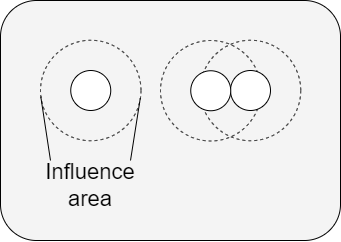
\includegraphics[width=\linewidth]{pics/interpersonal.drawio.png}
    \endminipage
    \caption{Interpersonal influence - Agents close enough to each other will influence each other's trust. On the right, two agents are close enough to update their trust levels between themselves.}
    \label{fig:interpersonal_influence}
\end{figure}
\begin{figure}[!htb]
    \centering
    \minipage{0.48\textwidth}
        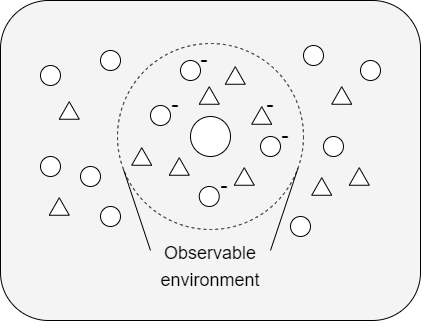
\includegraphics[width=\linewidth]{pics/observational.drawio.png}
    \endminipage
    \caption{Observational influence - Agents will observe their environment and update their own trust level based on their observations. The observing agent (big circle) can see four unvaccinated agents (small circles) with symptoms (\babelhyphen{nobreak}), five vaccinated agents (small triangles) without symptoms and one vaccinated agent with symptoms.}
    \label{fig:observational_influence}
\end{figure}

\clearpage

\begin{figure}[!htb]
    \centering
    \minipage{0.58\textwidth}
        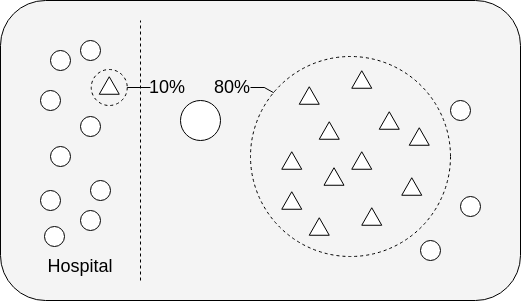
\includegraphics[width=\linewidth]{pics/institutional.drawio.png}
    \endminipage
    \caption{Institutional influence - Agents will receive information about the proportion of vaccinated agents in and out of a specific epidemiological state. The aware agent (big circle) is informed that 10\% of hospitalised agents are vaccinated and that 80\% of unhospitalised agents are vaccinated.}
    \label{fig:institutional_influence}
\end{figure}

\begin{figure}[!htb]
    \centering
    \minipage{0.34\textwidth}
        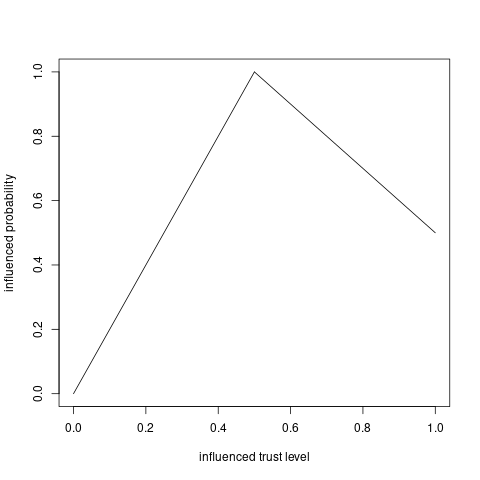
\includegraphics[width=\linewidth]{pics/influenced_probability.png}
        \caption{Probability to be influenced based on the influenced agent's trust level}
        \label{fig:influenced_probability}
    \endminipage
    \hspace{0.2in}
    \minipage{0.34\textwidth}
        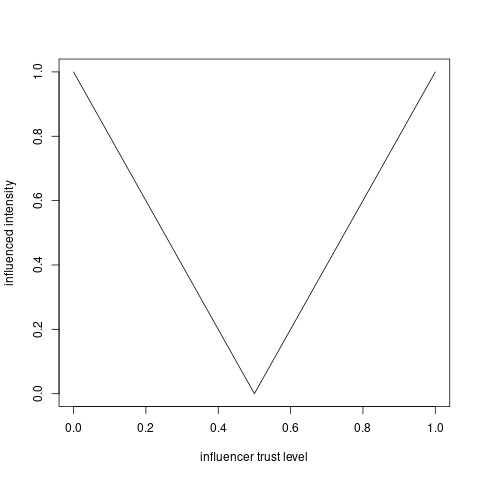
\includegraphics[width=\linewidth]{pics/influence_intensity.png}
        \caption{Intensity of the influence based on the influencer agent's trust level}
        \label{fig:influence_intensity}
    \endminipage
    \\
    \minipage{\textwidth}
        \centering
        \minipage{0.34\textwidth}
            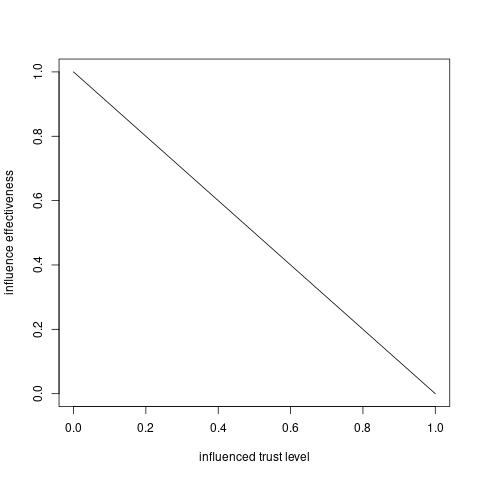
\includegraphics[width=\linewidth]{pics/influence_effectiveness_below.png}
        \endminipage
        \hspace{0.2in}
        \minipage{0.34\textwidth}
            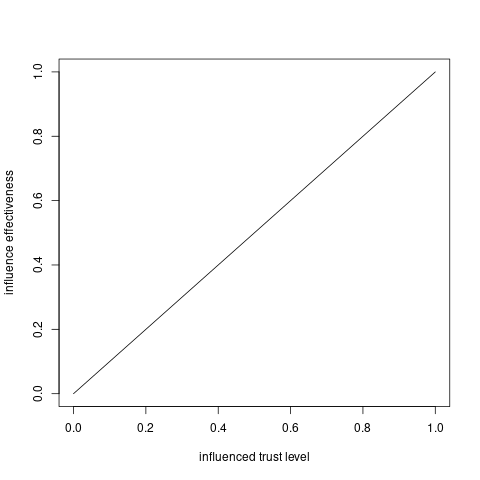
\includegraphics[width=\linewidth]{pics/influence_effectiveness_above.png}
        \endminipage
        \captionsetup{width=0.82\linewidth}
        \caption{Effectiveness of the influence based on the influenced agent's trust level whether the influencer agent's trust level is below 0.5 (left) or above 0.5 (right)}
        \label{fig:influence_effectiveness}
    \endminipage
\end{figure}

\pagebreak

\subsection{Interpersonal influence over trust}
When an agent comes into close contact with another agent upon entering a predefined influence area (figure \ref{fig:interpersonal_influence}) --- these areas surround each agent ---, it will be influenced by the other agent's trust level with a probability based on its own trust level. The other agent will obviously, in turn, be influenced by the first agent's trust level with a probability calculated similarly. See algorithm \ref{algo:interpersonal}.

Distrusting agents possess a trust level below 0.5. The probability $P(DI)$ for a distrusting agent to be influenced based on its trust level $tl$ is:
\[P(DI) = tl / 0.5\]

Trusting agents have a trust level above 0.5. The probability $P(TI)$ for a trusting agent to be influenced based on its trust level $tl$ is:
\[P(TI) = 0.5 + (1 - tl)\]

These two probabilities are represented in figure \ref{fig:influenced_probability} in which it is possible to see that in order to make distrusting agents (in range [0.0, 0.5[) less influenced than trusting agents (in range ]0.5, 1.0]), $P(DI)$ creates a linear probability distribution ranging from 0.0 to 1.0, while $P(TI)$ results in a linear probability distribution ranging from 0.5 to 1.0. This makes trusting agents susceptible to being influenced at least half of the time. If the probability is in favour of the influencer, a calculation is run to determine how much the trust level of the influenced agent is to be updated.

In order to determine the update to apply to the influenced agent's trust level, the intensity and the effectiveness of the influence need to be calculated. The intensity of the influence is based on the influencer's trust level and ranges piece-wise linearly from 0 to 1 for a trust level ranging from 0 to 0.5 and ranging from 0.5 to 1 (figure \ref{fig:influence_intensity}). The effectiveness of the influence is based on both the influencer agent's and the influenced agent's trust levels. If the influencer's trust level is below 0.5, then the influence effectiveness ranges linearly from 0 to 1 for an influenced trust level ranging from 1 to 0. If the influencer's trust level is above 0.5, then the influence effectiveness ranges linearly from 0 to 1 for an influenced trust level ranging from 0 to 1 (figure \ref{fig:influence_effectiveness}).

Once the intensity and the effectiveness calculated, the update to apply to the influenced agent's trust level is the multiplication of both, times -1 if the influencer agent's trust level is below 0.5.

\pagebreak

\begin{algorithm}[language=Pseudocode, caption={Interpersonal influence over trust}, label={pseudo_code_interpersonal}]
agents: list of all agents
get_alive_agents_in_contact(X): get all agents not deceased in agent X's surroundings within a fixed NetLogo radius of 0.1
random(f): produce a uniform distribution
begin
    for each influencer in agents do
        if not (influencer.is_hospitalised or influencer.is_deceased) then
            agents_in_contact <- get_alive_agents_in_contact(influencer)
            for each influenced in agents_in_contact do
                if influenced.trust_level < 0.5 then
                    probability_influenced <- random(influenced.trust_level / 0.5)
                else
                    probability_influenced <- random(0.5 + (1 - influenced.trust_level))
                end if
                if probability_influenced > random(1) then
                    if influencer.trust_level < 0.5 then
                        influence_intensity <- 1 - (influencer_trust_level / 0.5)
                        influence_effectiveness <- 1 - trust-level
                        influence_update <- influence_intensity * influence_effectiveness
                        influenced_trust_level <- influenced_trust_level - influence_update
                    else if influencer.trust_level > 0.5 then
                        influence_intensity <- (influencer_trust_level / 0.5) - 1
                        influence_effectiveness <- trust-level
                        influence_update <- influence_intensity * influence_effectiveness
                        influenced_trust_level <- influenced_trust_level + influence_update
                    else
                        influenced_trust_level <- influenced_trust_level
                    end if
                end if
            end for
        end if
    end for
end
\end{algorithm}

\begin{algorithm}[language=Pseudocode, caption={Observational influence over trust}, label={pseudo_code_observational}]
agents: list of all agents
get_alive_agents_in_surroundings(X): get all agents not deceased in agent X's surroundings within a fixed NetLogo radius of 0.5
begin
    for each observer in agents do
        if not (observer.is_hospitalised or observer.is_deceased) then
            agents_in_surroundings <- get_alive_agents_in_surroundings(observer)
            for each other in agents_in_surroundings do
                if other.is_vaccinated and not other.is_symptomatic then
                    observer.trust_level <- observer.trust_level + (0.03 * observer.trust_level)
                else if other.is_vaccinated and other.is_symptomatic then
                    observer.trust_level <- observer.trust_level - (0.05 * (1 - observer.trust_level))
                end if
            end for
        end if
    end for
end
\end{algorithm}

\subsection{Observational influence over trust}

Agents in a physical state that allows them to observe their environment will update their trust level based on their observation of vaccinated agents. Those observing agents are all agents, with exception to those having a Hospitalised or a Deceased epidemic state. There are two possible cases. If the observer agent sees a vaccinated and asymptomatic agent (other than in the Symptomatic or Hospitalised epidemic state), which is positive information, then its trust level will slightly increase. However, if the observer agent sees a vaccinated and symptomatic agent (in the Symptomatic or Hospitalised epidemic state), negative information, then its trust level will decrease more than in would have increased \cite{cvetkovich_new_2002}. These increases and decreases are small percentages (3\% and 5\%) of the observer agent's own trust level, working as a confirmation bias \cite{nickerson_confirmation_1998}. In addition, trusting agents will tend to ignore negative information as distrusting agents will tend to neglect positive information \cite{cvetkovich_new_2002}. See algorithm \ref{algo:observational}.

\subsection{Institutional influence over trust}
\label{conception_institutional}

Agents other than in a Hospitalised or Deceased epidemiological state will get their trust level updated according to the received information and their own trust level. In order to update all attentive agents' trust level, (a) the proportion of vaccinated agents among the epidemiological state of concern and (b) the proportion of all other alive vaccinated agents in the environment must first be calculated. The difference between those two proportions (b - a) --- divided by 1000 to lighten its effect --- is then used to create the value by which to update. If the difference is above 0, the type of the information is considered positive. If the difference is below 0, the type of the information is considered negative. The difference is then attenuated and adjusted with each agent's trust level depending on the information type (confirmation bias \cite{nickerson_confirmation_1998}) before finally becoming the update value to apply independently to each agent. Additionally, the option to make that information incomplete was added. See algorithm \ref{algo:institutional}.

\begin{algorithm}[language=Pseudocode, caption={Institutional influence over trust}, label={pseudo_code_institutional}]
agents: list of all agents
proportion_X_vaccinated: percentage of vaccinated among agents with an epidemiological state X
proportion_not_X_vaccinated: percentage of vaccinated not among agents with an epidemiological state X
begin
    for each agent in agents do
        if not (agent.is_hospitalised or agent.is_deceased) then
            if agent.misinterprets then
                trust_level_update <- (proportion_X_vaccinated / 100) * -1 * (1 - agent.trust_level)
            else
                proportion_difference <- (proportion_not_X_vaccinated - proportion_X_vaccinated) / 100
                if proportion_difference >= 0 then
                    trust_level_update <- proportion_difference * 0.5 * agent.trust_level
                else
                    trust_level_update <- proportion_difference * (1 - agent.trust_level)
                end if
            end if
            agent.trust_level <- agent.trust_level + trust_level_update
        end if
    end for
end
\end{algorithm}

\chapter{Implementation}

The implementation of the presented simulation is based on a previous simulation that can be found on the CoVprehension website \cite{covprehension_question_17_2020, adam:hal-03613433}. CoVprehension is a project independent of any organisation and initiated by researchers during the COVID-19 pandemic. The goal of this project is not to predict, but to explain in a simple way, with a scientific background, the evolution of the epidemic and its potential outcomes. In order to achieve this goal, different stages of the epidemic and ideas on how to battle it have been summarised into questions which, in turn, lead to explanations accompanied by sketches, diagrams and interactive simulations.

The previous simulation took as basis question 17 of CoVprehension \cite{covprehension_question_17_2020}: "Let{\textquoteright}s test people! Sure, but who, when and how?" Simply put, it shows how handling the epidemic through the use of screening tests is far from easy. Depending on the testing strategy, the constraint of limited available test kits and the delayed start of the campaign, different outcomes are obtained and may lead to decisions based on insufficient data.

Some changes were made to this previous simulation of question 17. Looking at the epidemiological model, the Incubation state was removed, and two new states were added: Hospitalised and Deceased. The Incubation state is not needed as it cancels itself out when updating trust levels and would bring, in this simulation, a useless delay before changing into a Symptomatic or an Asymptomatic state.
Within agents' attributes, everything related to testing and quarantine was removed, while a vaccination status and a trust level attribute were added. Keeping the testing and the quarantine parameters would have lengthened the duration of the simulation and over-complicated it. Instead, agents will directly know in which epidemiological state they and others are (except for asymptomatic agents, which are viewed and mistaken as susceptible agents). Finally, a number of methods were added, mostly in order to create a hospitalised area with visiting agents and interactions to update trust levels.

The source code, excluding the graphics user interface, is made of approximately 800 lines and is available on GitHub.\footnote{Source code: \url{https://github.com/CalvinMT/TrustVaccSim}} It was implemented and tested on NetLogo 6.2.2 using a 4 core CPU for which attaining 100 simulation ticks at normal simulation speed took around 7 seconds. Running the same code on NetLogo Web is possible\footnote{Simulator on NetLogo Web: \url{https://www.netlogoweb.org/launch\#https://raw.githubusercontent.com/CalvinMT/TrustVaccSim/main/src/trustvaccsim.nlogo}}, yet slower, reaching 100 simulation ticks with a normal simulation speed at around 23 seconds. A screenshot of the simulation on NetLogo Web can be viewed in figure \ref{fig:simulation_screenshot}.


\section{Simulation specifications}

\begin{figure}
    \centering
    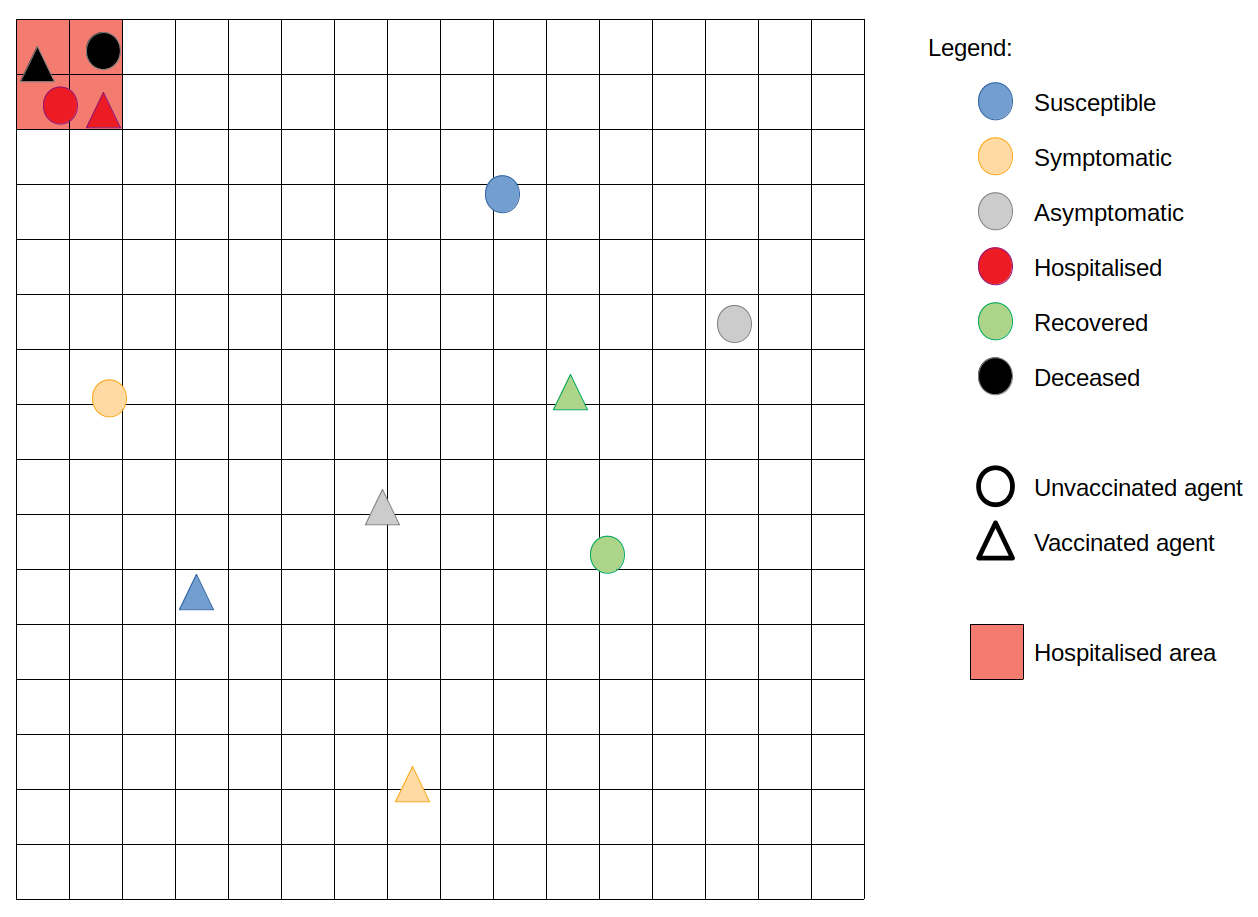
\includegraphics[width=0.9\linewidth]{pics/simulation_figure.png}
    \caption{Visual outline of the environment of the simulator.}
    \label{fig:simulation_environment}
\end{figure}

The environment of the simulation consists of a square of 256 patches (16x16) in which a population of 2000 agents is equally distributed between all patches other than those considered the hospitalised area. The hospitalised area is situated in the top-left corner of the environment and takes up a square of 4 patches (2x2). Simply put, a patch, in NetLogo, is a square with accessible properties that composes the environment on which agents can wander and perform their activities.

Each agent starts in the Susceptible state, with exception to one randomly chosen agent initialised with the Symptomatic state. Once the simulation starts, agents move around freely and randomly in the environment, avoiding the hospitalised area. Agents on the same patch are considered close enough for airborne transmission of the virus, as through the means of aerosols. Thus, if one of them is infectious, other agents on the same patch and in the Susceptible state have a risk of getting infected, putting them either in the Symptomatic or Asymptomatic state. If in the Hospitalised state, agents are moved into the hospitalised area, as if taken into a hospital. They will stay in that area without infecting anyone until they recover from the disease. Hospitalised agents are visited by ten other randomly chosen non-hospitalised agents for 5 simulation steps.

An agent's colour informs the user of the simulation on its epidemiological state, while its shape notifies on its vaccination status. Blue is Susceptible, yellow is Infected, grey is Asymptomatic, red is Hospitalised, green is Recovered and black is Deceased. Once an agent falls into the Deceased state, it stops moving and vanishes over time. As agents pop in and out of the hospitalised area, the choice was made to make agents that fall into the Deceased state gradually vanish instead of directly disappear so that the user can clearly identify when agents go from a Hospitalised state to a Deceased state. Additionally, they are not left visible in the simulation, or they would, in some scenarios, rapidly fill the hospitalised area. Concerning the vaccination status, an agent represented as a circle is unvaccinated and an agent drawn as a triangle is vaccinated.
A visual outline of the environment of the simulator is observable in figure \ref{fig:simulation_environment}.


\section{Entry parameters}
\label{entry_parameters}

The simulation enables users to modify a single of its entry parameters. This simplicity in the simulation allows the user to focus solely on the effect of this parameter alone over the entire model, thus making it easier for the user to observe what the simulator is intended to show them.

The modifiable entry parameter is the initial average trust of the population. This parameter is identified as a slider ranging from 0.1 to 0.9 with steps of 0.1. A population with an average trust of 0.1 is considered representative of a highly distrusting population, while a population considered highly trusting would have an average trust of 0.9. This average trust is initialised using a custom distribution algorithm as shown in figure \ref{fig:initial_average_trust}. This method was chosen for its simple implementation and in order not to limit the range of randomly chosen trust levels as a normal distribution would, but closer to what a skew normal distribution would give.

\begin{figure}[!htb]
    \centering
    \minipage{0.6\textwidth}
        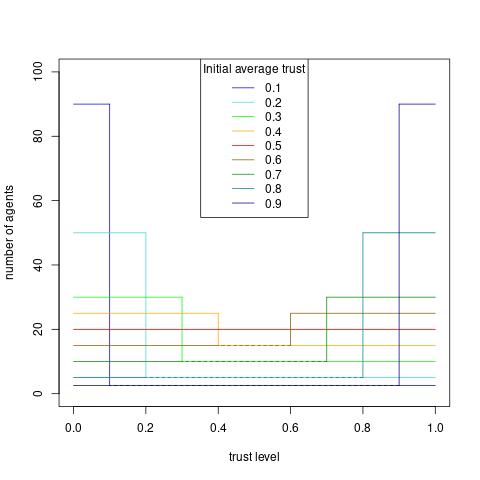
\includegraphics[width=\linewidth]{pics/initial_average_trust.png}
        \caption{Output of the algorithm used in the initialisation of the population's average trust.}
        \label{fig:initial_average_trust}
    \endminipage{}
\end{figure}

\pagebreak

The idea behind the trust level initialisation algorithm is simple and goes as follows. For all agents, if the current population's average trust --- a floating point initialised at 0 --- is below the user-set initial population's average trust, then the trust level of the current agent is randomly set between $X$ and 1. $X$ being the opposite number to the current population's average trust level, based on the user-set initial average trust level. Although, if $X$ is above 1, it is set to 0.9. And if $X$ is below 0, it is set to 0.1. Otherwise, if the current population's average trust is above the user-set initial population's average trust, this time the current agent's trust level is randomly set between 0 and $X$. Finally, if the current population's average trust is equal to the user-set initial population's average trust, the current agent's trust level is set between 0 and 1. See algorithm \ref{algo:initialisation_trust_level}.


\section{Outputs}
\label{implementation_outputs}

The user can visualise the environment in which agents wander around. This enables the user to observe agents changing from one epidemiological state to another by their colour and change vaccination status by their shape. Through this visualisation, the user can identify if the hospitalised area is more or less crowded.

A number of graphical outputs are also displayed to the user in order to follow the evolution of different variables:
\begin{itemize}
    \item Epidemic dynamic --- Percentage of agents over time for all epidemiological states, as well as the percentage of vaccinated agents over time and the average trust level of the population.
    \item Level of trust per interpretation status --- Average trust level of the correctly interpreting population and incorrectly interpreting population over time.
    \item Deaths per vaccination and interpretation statuses --- Number of deceased, unvaccinated and misinterpreting agents over time with the number of deceased, unvaccinated and correctly interpreting agents over time next to the number of deceased, vaccinated and misinterpreting agents over time followed by the number of deceased, vaccinated and correctly interpreting agents over time.
\end{itemize}

These visualisations were chosen to enable the user to make multiple key observations aiming at the goal of the present work. The user may observe the evolution of the epidemic, of the vaccination campaign, and of the population's average trust with the help of the epidemic dynamic. The observation of the average trust level between two subgroups of the population having different interpretation of information may assist the user in understanding the influence of misinterpretation of information on the population's average trust level, as well as the differences in starting an epidemic with a high or a low population's average trust level. Finally, observing the sorted death rate may help the user appreciate the resulting effect of having incorrectly interpreted information, having been vaccinated or not.
\chapter{Results}

\section{Design of experiments}

Because agent-based models are stochastic and that random functions are used in the simulation model's implemented algorithms, there is a need to compute multiple simulations and to average their outputs. NetLogo includes a design of experiments framework called "BehaviorSpace" which allows for a succession of experiments to be run successively, each starting with a set of different entry parameter values. The only input parameter to change with this simulation is the population's initial average trust. This parameter will change starting from 0.1 and ending at 0.9 with steps of 0.1. As the model has random factors, the simulation will be run 100 times at each parameter step in order to average out output values.
The experiment has six outputs, which are those used to create two of the output graphs in section \ref{implementation_outputs}: two outputs for the trust level per misinterpretation status, and four outputs for the number of Deceased per vaccination and misinterpretation statuses. These outputs contain the information needed to make the wanted observations. Once all experiments performed and terminated --- which took approximately fifteen minutes on a four core CPU ---, a Python script helped to combine the different experiment outputs into average values which were then plotted to obtain figures \ref{fig:dvm} and \ref{fig:tm}.

It can directly be observed in both figures that starting with a low population's initial average trust, such as 0.1, 0.2 and 0.3, shortens the duration of the simulation. This is explained by the fact that, when more agents distrust than trust, less of them get vaccinated, resulting in more deaths. Conversely, when more agents trust than distrust, more of them get vaccinated and less of them fall into the Deceased state.

Another characteristic to be pointed out from both figures is the high irregularity near the end of the timeline of the different plots, especially those with a low population initial average trust level. These fluctuations at the end of the different curves are a result of averaging out less simulations. As most simulations finish at an earlier time step, fewer of them continue running, reaching a higher time step.
This could be avoided either by running simulations with the same input parameter a greater number of times, or by stopping the simulations at a specified time step.



\section{Results analysis}
\label{results_analysis}

\subsection{Trust and misinterpretation}

Figure \ref{fig:tm} shows, with two curves, the evolution in time of the population average trust level during the simulation for each value of the population's trust level entry parameter. One curve represents the average trust level of the population correctly interpreting the information given through the institutional influence interaction from section \ref{conception_institutional}. And the other curve represents the average trust level of the population incorrectly interpreting (misinterpreting) the information given through the same interaction. See figure \ref{fig:tm_landscape} in appendix for a wider version.

From this figure, it is possible to see that:
\begin{enumerate}
    \item The average trust of the part of the population that interprets correctly the information given to them increases faster than for the part of the population that interprets incorrectly the same information.
    \item The higher the population's initial average trust is, the faster the increase in trust, and the less difference there is in trust between parts of the population that interpret the information correctly versus incorrectly.
\end{enumerate}

\begin{figure}[!htb]
    \centering
    \minipage{0.78\textwidth}
        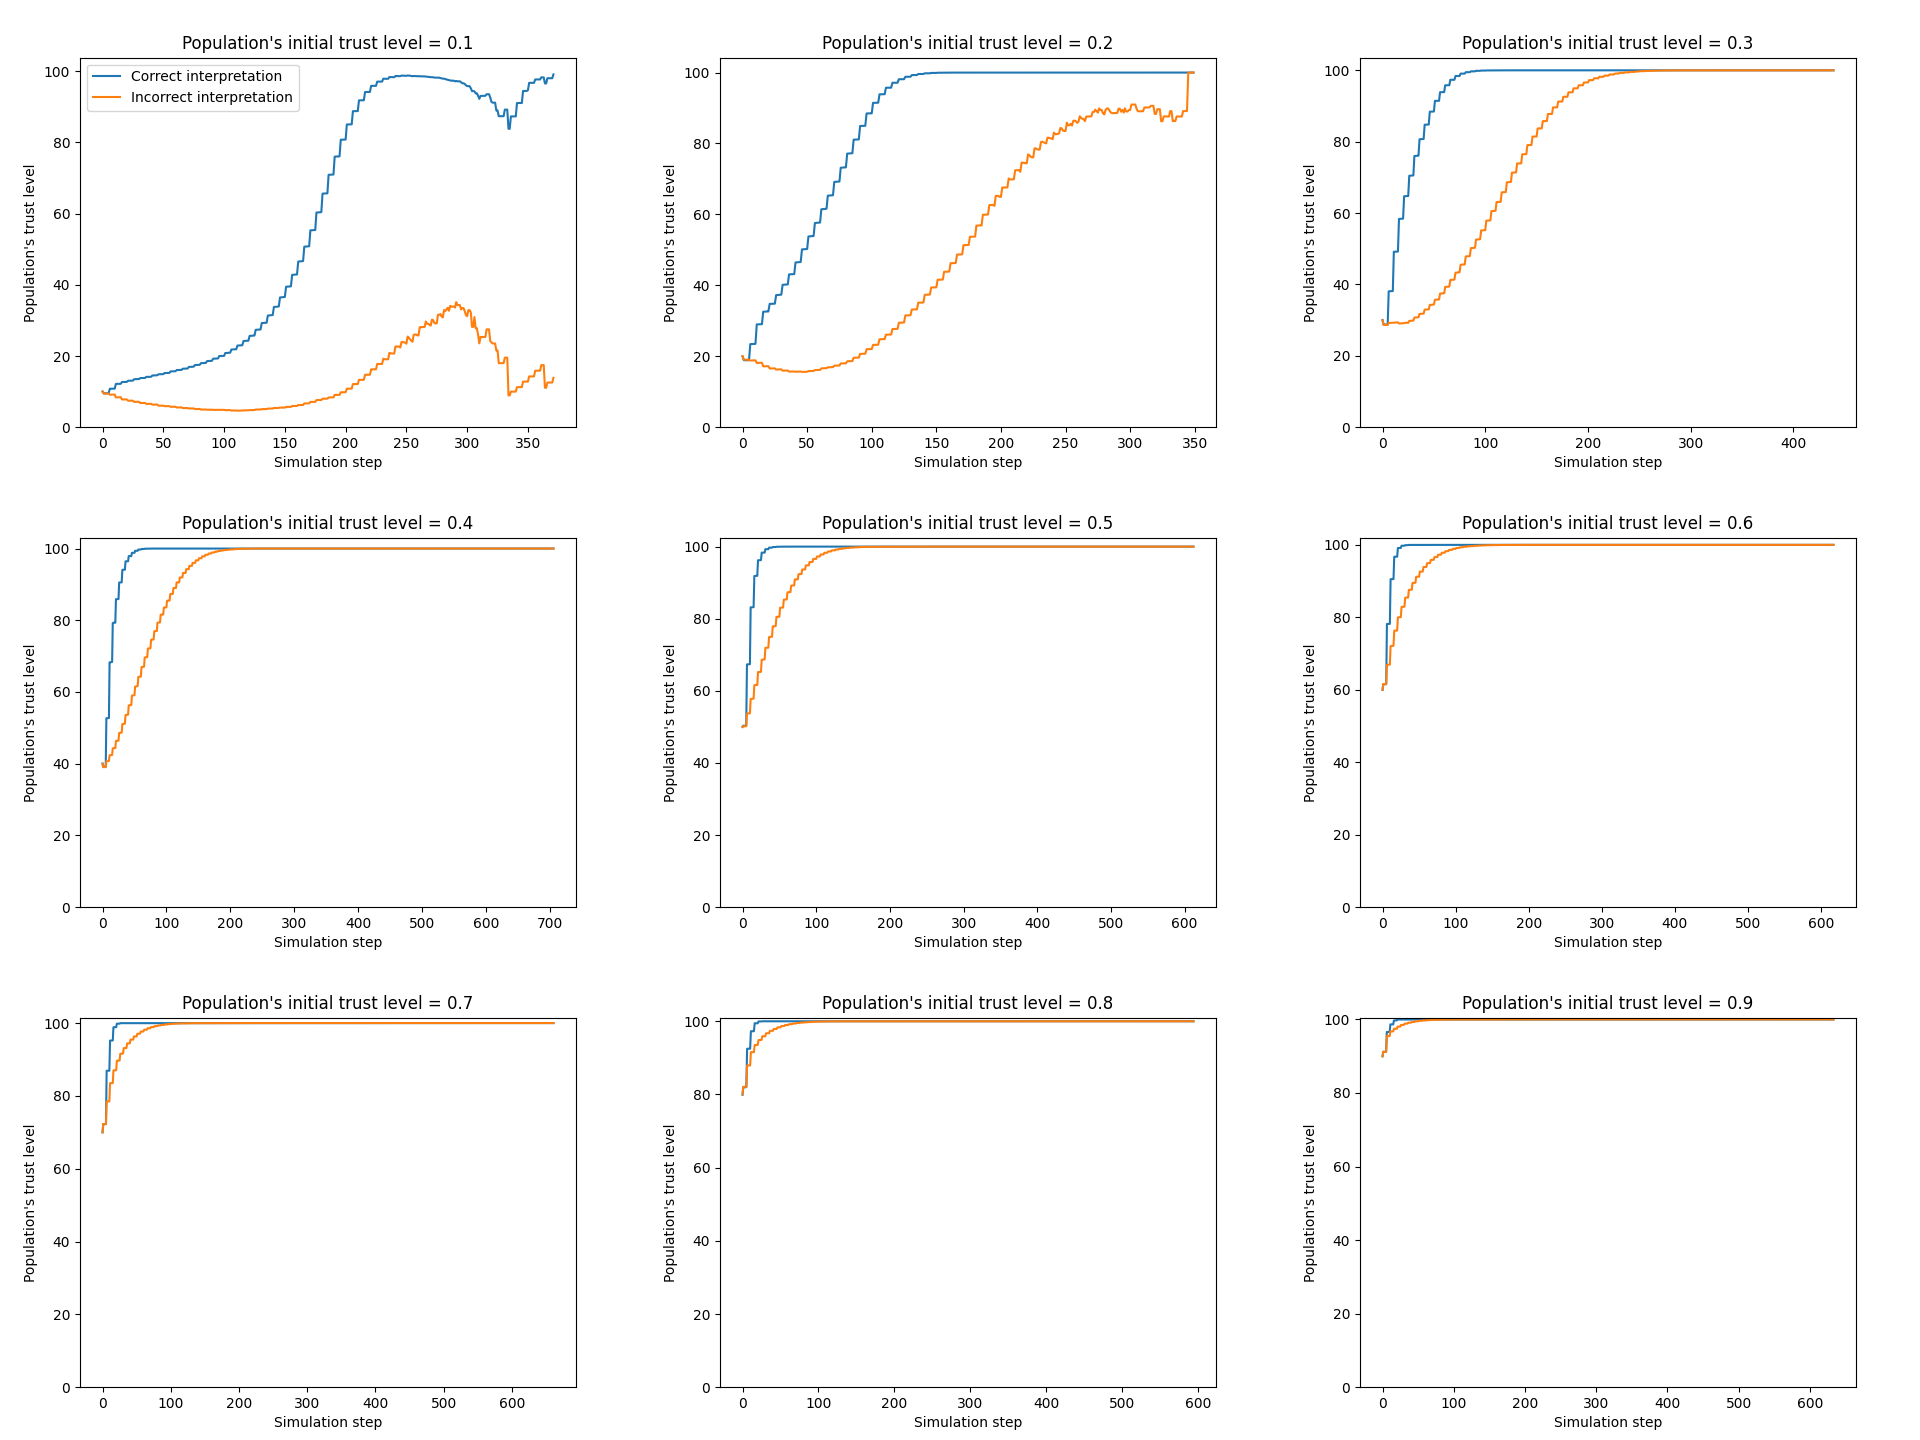
\includegraphics[width=\linewidth]{pics/TM.png}
    \endminipage{}
    \caption{Average population's trust level per misinterpretation status at each simulation step for each population's initial trust level. The number of simulation steps (x-axis) is different between graphs.}
    \label{fig:tm}
\end{figure}

\pagebreak

\subsection{Deceased, vaccinated and misinterpretation}

Figure \ref{fig:dvm} shows, with four curves, the evolution in time of the number of agents in the Deceased state per vaccination and misinterpretation statuses for each value of the population's trust level entry parameter. The first curve represents the number of agents which deceased being unvaccinated and interpreting the given information correctly. The second curve represents the number of agents which deceased being unvaccinated and interpreting the given information incorrectly. The third curve represents the number of agents which deceased being vaccinated and interpreting the given information correctly. Finally, the fourth curve represents the number of agents which deceased being vaccinated and interpreting the given information incorrectly. See figure \ref{fig:dvm_landscape} in appendix for a wider version.

From this figure, it is possible to see that:
\begin{enumerate}
    \item Reported agents with a Deceased state are mainly unvaccinated agents, as vaccinated agents are almost always reported to be 0. This is due to the choice to configure the model's vaccine as a highly effective vaccine (see section \ref{concept_vaccination_status}).
    \item There is a distinct gap between both unvaccinated groups of now deceased agents when the population's initial average trust is low, even average (from 0.1 to 0.5 included). This gap tends to shrink as the population's initial average trust gets higher. It is clear that unvaccinated agents misinterpreting information given to them have a higher death rate than those having a correct interpretation of the same information when the average trust of the population is low. In other words, a high population's initial average trust tends to negate the effect of misinterpretation.
\end{enumerate}

\begin{figure}[!htb]
    \centering
    \minipage{0.78\textwidth}
        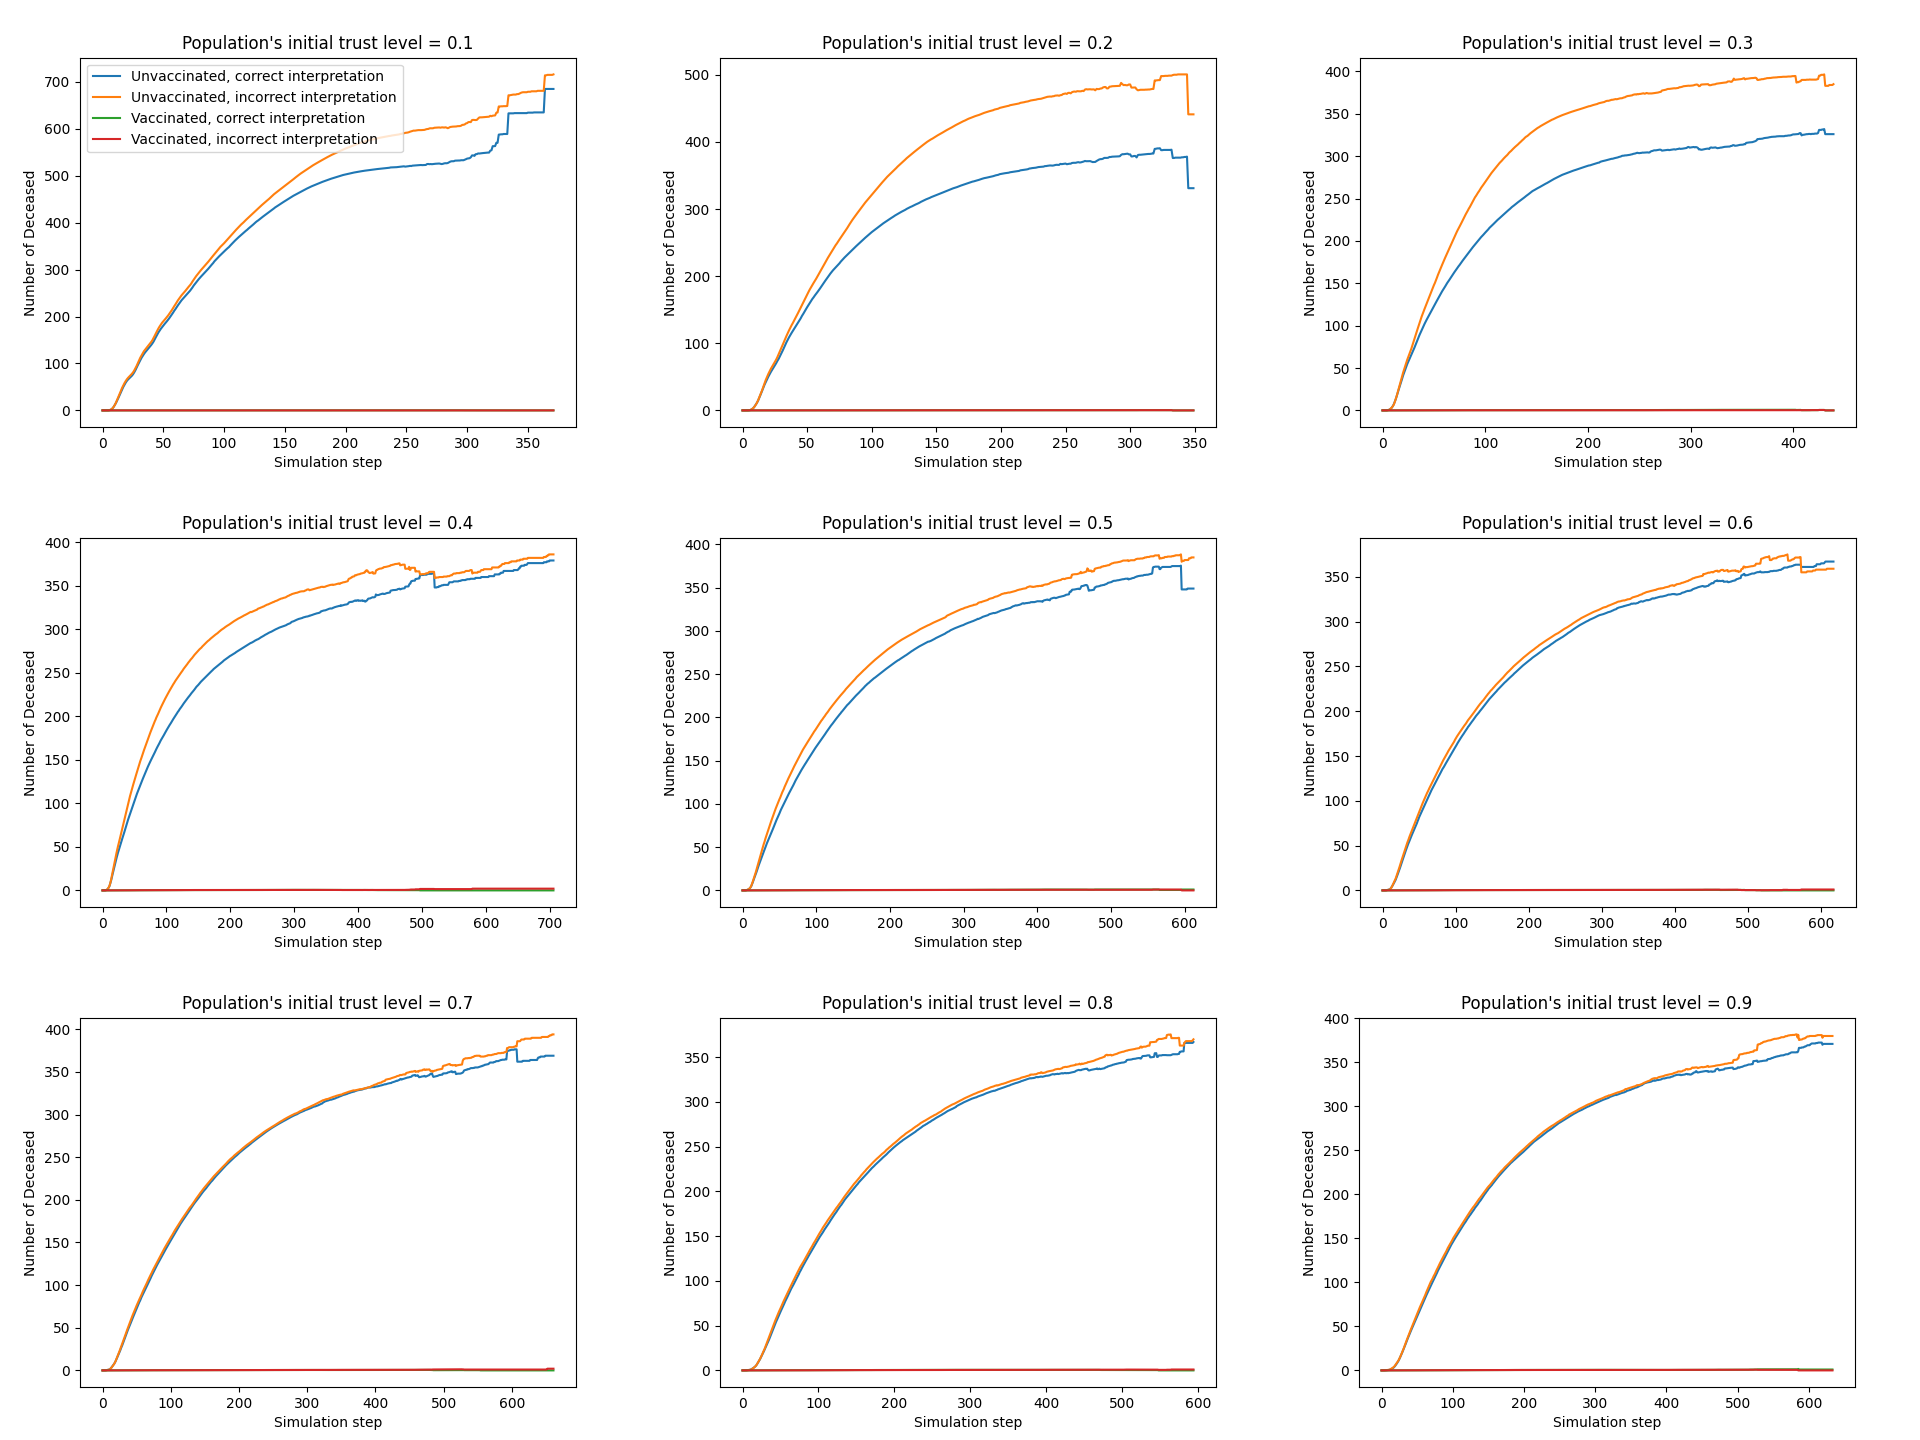
\includegraphics[width=\linewidth]{pics/DVM.png}
    \endminipage{}
    \caption{Average number of deaths per vaccination and misinterpretation statuses at each simulation step for each population's initial trust level. The number of simulation steps (x\babelhyphen{nobreak}axis) is different between graphs.}
    \label{fig:dvm}
\end{figure}

\chapter{Discussion}

To build an educational simulation with an agent-based model of an epidemic with vaccination and trust, a lot of knowledge had to be gathered through research within various disciplines. Doing so allowed the implementation of an SIAHRD epidemiological model and helped with the application of a vaccination status, as well as with the addition of a trust human behaviour attribute and its methods.

Although the results look concluding, logical and seem close enough to realistic for an educational simulation, it is hard to find any data that could validate them. One way that the results could be validated would be to have them examined by epidemiologists and psychologists.
Additionally, and as noticeable in section \ref{results_analysis}, various observations can be made. Thus, there is a need to run a proper experimentation with participants in order to see if the different expected observations are understood by various members of the public.



\section{Future plans}

Not everything thought of during the time taken to focus on the present work could be implemented. The subject is as deep as the researcher wants it to be and data to attain the desired goal is scattered between scientific articles, news journals, independent websites and social media. However, here are a few ideas to continue on the course of this work.

One could consider making the environment of the simulation a town or a city with households \cite{grignard_gama_2013}. Influence within those households would make it possible to view greater changes in trust and vaccination in some parts of the environment than others.
Additionally, hospital visits would be organised differently, as only members of a same household would visit hospitalised agents.

Incorporating age groups would allow implementing family influence over trust. This could be important as children are more than often influenced by their parents \cite{sheehan_trust_2020}. Additionally, younger generations are more inclined to show refusal and delay in vaccine intake \cite{soares_factors_2021}.

Extending the model with different information source types (government documents, medical recommendations, or social media) could influence the trust level of agents in more diverse ways, as it has been reported that, younger generations tend to get their information on social media more than other generations \cite{okeeffe_impact_2011, roozenbeek_susceptibility_2020}.



\section{End note}

Even if vaccination becomes mandatory, if a population does not show trust, may it be in vaccines in general or in the government, people will find ways to get around policies they do not feel trustworthy. Reports of people getting fake vaccine passes and health care assistants providing counterfeit vaccine injections were making news during the SARS-CoV-2 epidemic \cite{davies_fake_covid_passes_2021, cnn_germany_fake_vaccines_2021, tondo_italy_fake_vaccines_2022}.
To prevent such behaviours, political and medical authorities should constantly double their efforts in correcting misinformation and countering disinformation \cite{abd-alrazaq_top_2020}. However, increase of trust should be sought prior to these efforts, which might even prevent them from being required.
In parallel, citizens must appreciate the importance of questioning gathered information with conscious humility to avoid any misinterpretation which could lead, as the present work attempted to show, to irreversible and tragic events.

\appendix \chapter{Appendix}
\label{chap:appendix}

\begin{algorithm}[language=NetLogo, caption={Interpersonal influence over trust}, label={algo:interpersonal}]
;; update agents' trust level when in contact with each other
to interpersonal-influence-over-trust
  ask turtles with [epidemic-state != "Hospitalised" and epidemic-state != "Deceased"] [
    let influencer-trust-level trust-level
    ask other turtles in-radius 0.1 with [epidemic-state != "Deceased"] [
      let proba-influ (ifelse-value
        ;; non-trusting agents are less influenced than trusting agents
        trust-level < 0.5 [ random-float trust-level / 0.5 ]
        [ random-float (1 - trust-level) + 0.5 ]
      )
      if random-float 1 < proba-influ
      [
        ;; influence trust
        (ifelse
          influencer-trust-level < 0.5
          [
            ;; influencer's trust level of 0.0 has an intensity of 1
            let influencer-influence-intensity 1 - (influencer-trust-level / 0.5)
            ;; high effectiveness on trust level 0.0 (low on 1.0)
            let influence-effectiveness 1 - trust-level
            let influence-update influencer-influence-intensity * influence-effectiveness
            set trust-level trust-level - influence-update
            if trust-level < 0 [ set trust-level 0 ]
          ]
          influencer-trust-level > 0.5
          [
            ;; influencer's trust level of 1.0 has an intensity of 1
            let influencer-influence-intensity (influencer-trust-level / 0.5) - 1
            ;; high effectiveness on trust level 1.0 (low on 0.0)
            let influence-effectiveness trust-level
            let influence-update influencer-influence-intensity * influence-effectiveness
            set trust-level trust-level + influence-update
            if trust-level > 1 [ set trust-level 1 ]
          ]
          ;; else influencer-trust-level == 0.5
          ;; influencer's trust level of 0.5 has an intensity of 0
        )
      ]
    ]
  ]
end
\end{algorithm}

\newpage

\begin{algorithm}[language=NetLogo, caption={Observational influence over trust}, label={algo:observational}]
;; update agents' trust level according to the infectious & vaccination status of agents around them (as well as themselves)
to observational-influence-over-trust
  if on-going-vaccination?
  [
    ask turtles with [epidemic-state != "Hospitalised" and epidemic-state != "Deceased"] [
      let observer-update 0
      ask other turtles in-radius 0.5 with [epidemic-state != "Deceased"] [
        let is-other-vaccinated? vaccinated?
        let is-other-symptomatic? ((epidemic-state = "Infected") or (epidemic-state = "Hospitalised"))
        ;; negative information have more impact than positive information
        (ifelse
          is-other-vaccinated? and (not is-other-symptomatic?)
          [
            ;; positive information
            set observer-update observer-update + (0.03 * trust-level)
          ]
          is-other-vaccinated? and is-other-symptomatic?
          [
            ;; negative information
            set observer-update observer-update - (0.05 * (1 - trust-level))
          ]
        )
      ]
      set trust-level trust-level + observer-update
      if trust-level < 0 [ set trust-level 0 ]
      if trust-level > 1 [ set trust-level 1 ]
    ]
  ]
end
\end{algorithm}

\newpage

\begin{algorithm}[language=NetLogo, caption={Institutional influence over trust}, label={algo:institutional}]
;; update agents' trust level comparing the percentage of agents in epidemiologic state X with the percentage of agents not in the epidemiologic state X
to institutional-influence-over-trust [nb-X nb-X-V is-X-D?]
  if on-going-vaccination? and nb-X > 0
  [
    ;; percentage of vaccinated among X
    let prop-X-V nb-to-prop nb-X-V nb-X
    ;; percentage of vaccinated not among X
    let prop-nX-V 0
    ifelse is-X-D?
      [set prop-nX-V nb-to-prop (total-vaccinations - nb-X-V) (population-size - nb-X)]
      [set prop-nX-V nb-to-prop (total-vaccinations - nb-X-V) (population-size - nb-X - nb-D)]
    ask turtles with [epidemic-state != "Hospitalised" and epidemic-state != "Deceased"] [
      let trust-level-update 0
      ;; institutional influence with a lack of knowledge or difficulties understanding statistics
      ifelse misinterpret? [
        set trust-level-update (prop-X-V / 100) * -1 * (1 - trust-level)
      ]
      ;; institutional influence with complete knowledge and understanding of statistics
      [
        let prop-nX-X-V-difference (prop-nX-V - prop-X-V) / 100

        ifelse prop-nX-X-V-difference >= 0 [
          ;; positive information is attenuated (* 0.5)
          ;; non-trusting agents will tend to neglect the positive information
          set trust-level-update prop-nX-X-V-difference * 0.5 * trust-level
        ]
        [
          ;; trusting agents will tend to neglect the negative information
          set trust-level-update prop-nX-X-V-difference * (1 - trust-level)
        ]
      ]
      set trust-level trust-level + trust-level-update
      if trust-level < 0 [ set trust-level 0 ]
      if trust-level > 1 [ set trust-level 1 ]
    ]
  ]
end
\end{algorithm}

\newpage

\begin{algorithm}[language=NetLogo, caption={Initialisation of the population's trust level}, label={algo:initialisation_trust_level}]
;; initialisation of each agent's trust level
to setup-population-trust-level
  ;; number of currently initialised agents' trust
  let current-trust-average-count 0
  ask turtles
  [
    (ifelse
      ;; if current population's average trust is below initial trust level
      ;; set trust level between X and 1
      ;; X = opposite number to current average of population trust based on initial trust level
      current-trust-average < initial-trust-level
      [
        let trust-average-adjuster (initial-trust-level + (initial-trust-level - current-trust-average))
        if trust-average-adjuster > 1
        [
          set trust-average-adjuster 0.9
        ]
        set trust-level trust-average-adjuster + (random-float (1 - trust-average-adjuster))
      ]
      ;; if current population's average trust is above initial trust level
      ;; set trust level between 0 and X
      ;; X = opposite number to current average of population trust based on initial trust level
      current-trust-average > initial-trust-level
      [
        let trust-average-adjuster (initial-trust-level - (current-trust-average - initial-trust-level))
        if trust-average-adjuster < 0
        [
          set trust-average-adjuster 0.1
        ]
        set trust-level random-float trust-average-adjuster
      ]
      ;; if current average of population trust is equal to initial trust level
      ;; set trust level between 0 and 1
      [
        set trust-level random-float 1
      ]
    )

    set current-trust-average-count current-trust-average-count + 1
    set current-trust-average (current-trust-average * (current-trust-average-count - 1) / current-trust-average-count + trust-level / current-trust-average-count)
  ]
end
\end{algorithm}

\newpage

\begin{figure}[!htb]
    \centering
    \minipage{\textwidth}
        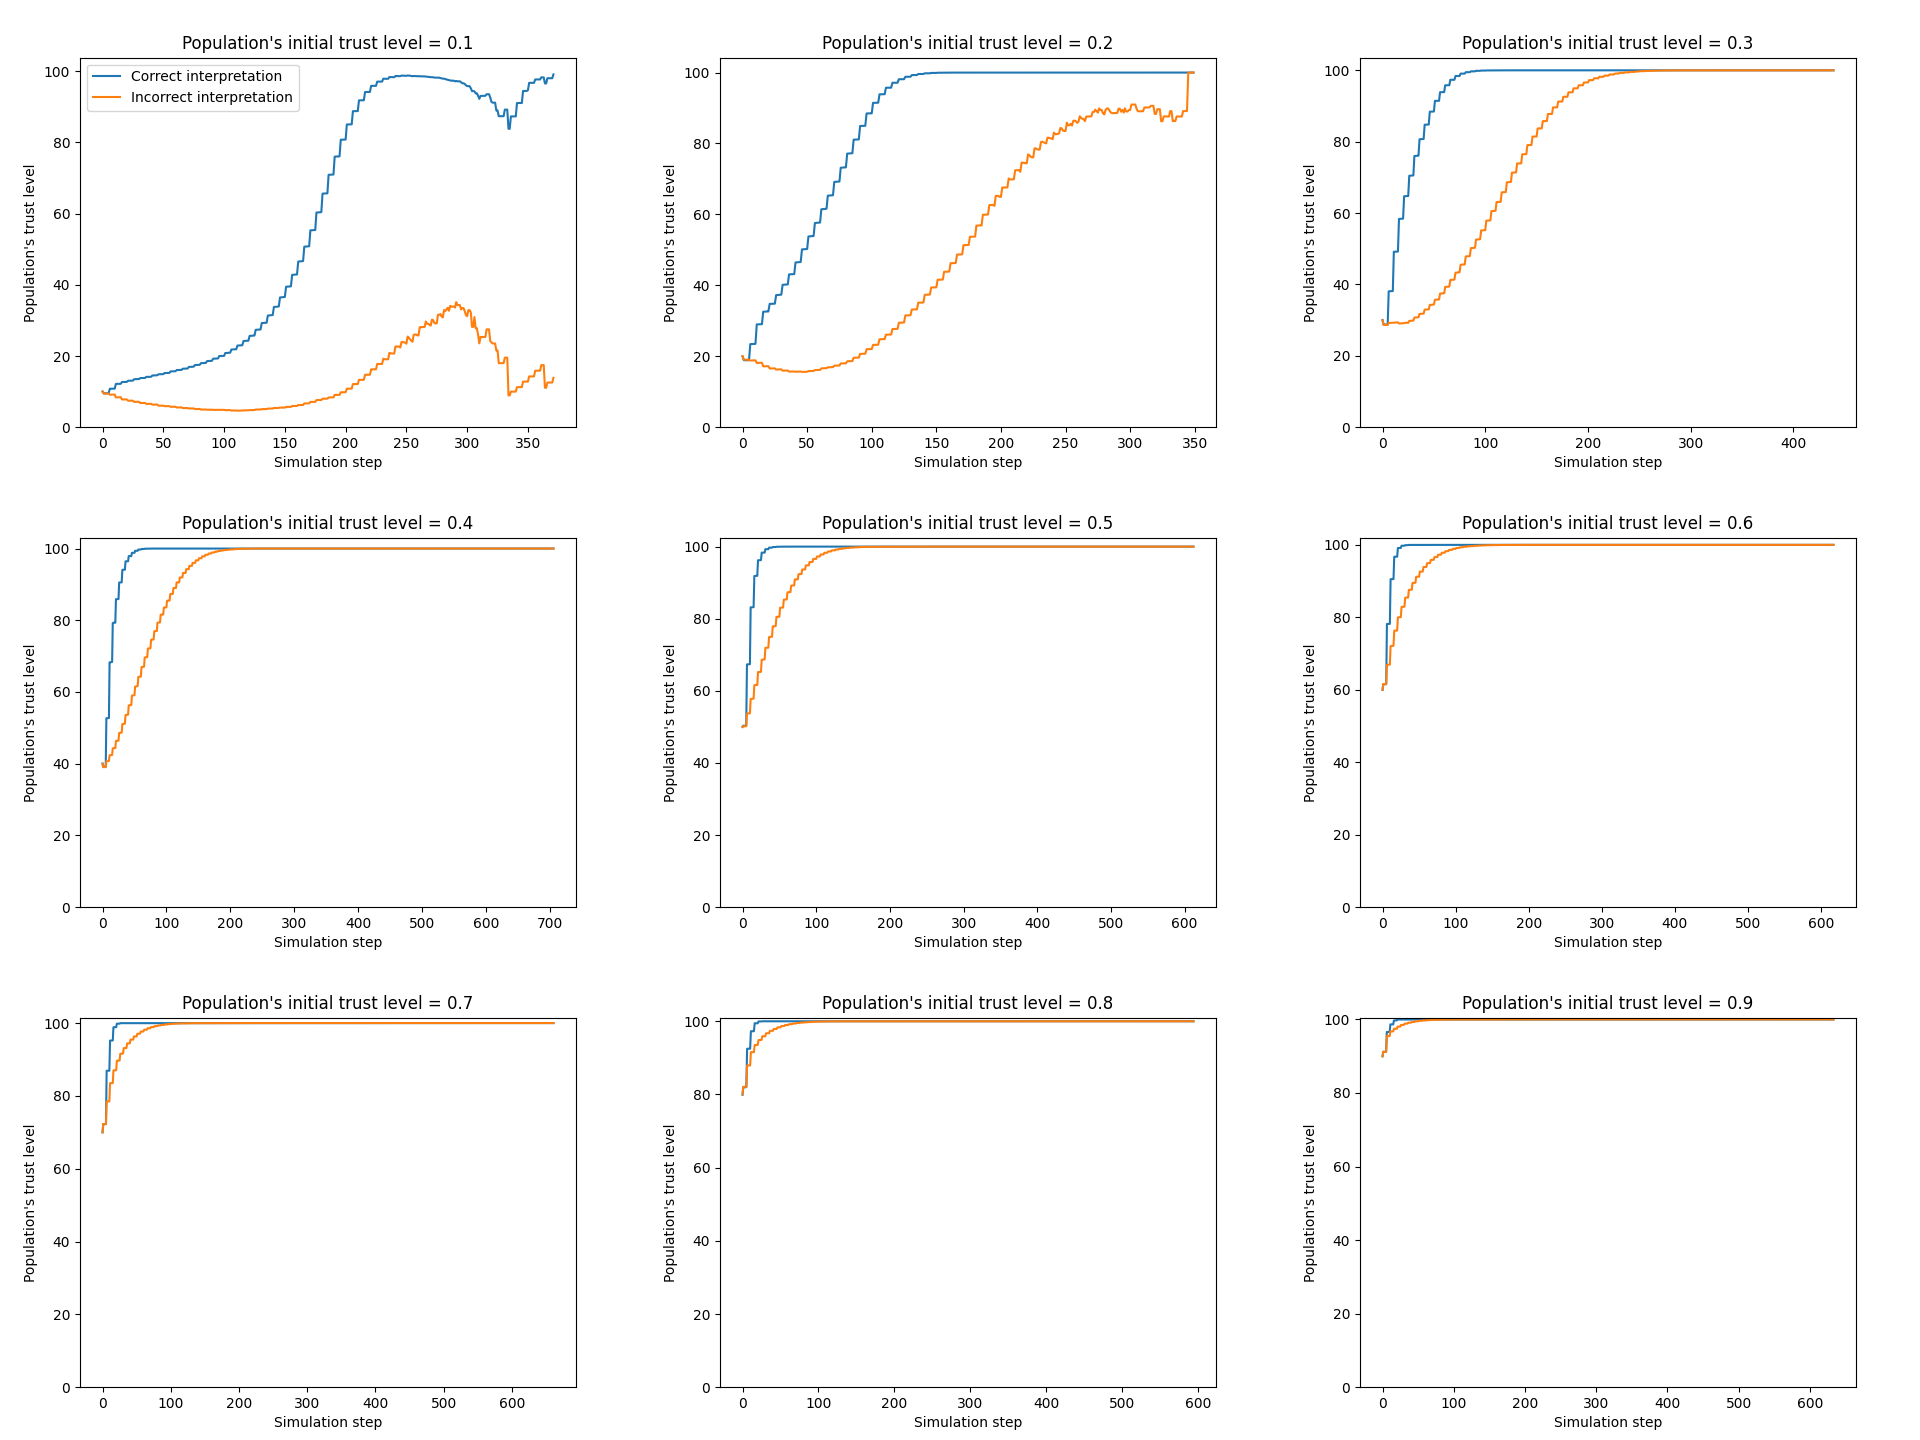
\includegraphics[width=1.3\linewidth, angle=90, origin=c]{pics/TM.png}
    \endminipage
    \caption{Average population's trust level per misinterpretation status at each simulation step for each population's initial trust level. The number of simulation steps (x-axis) is different between graphs.}
    \label{fig:tm_landscape}
\end{figure}

\newpage

\begin{figure}[!htb]
    \centering
    \minipage{\textwidth}
        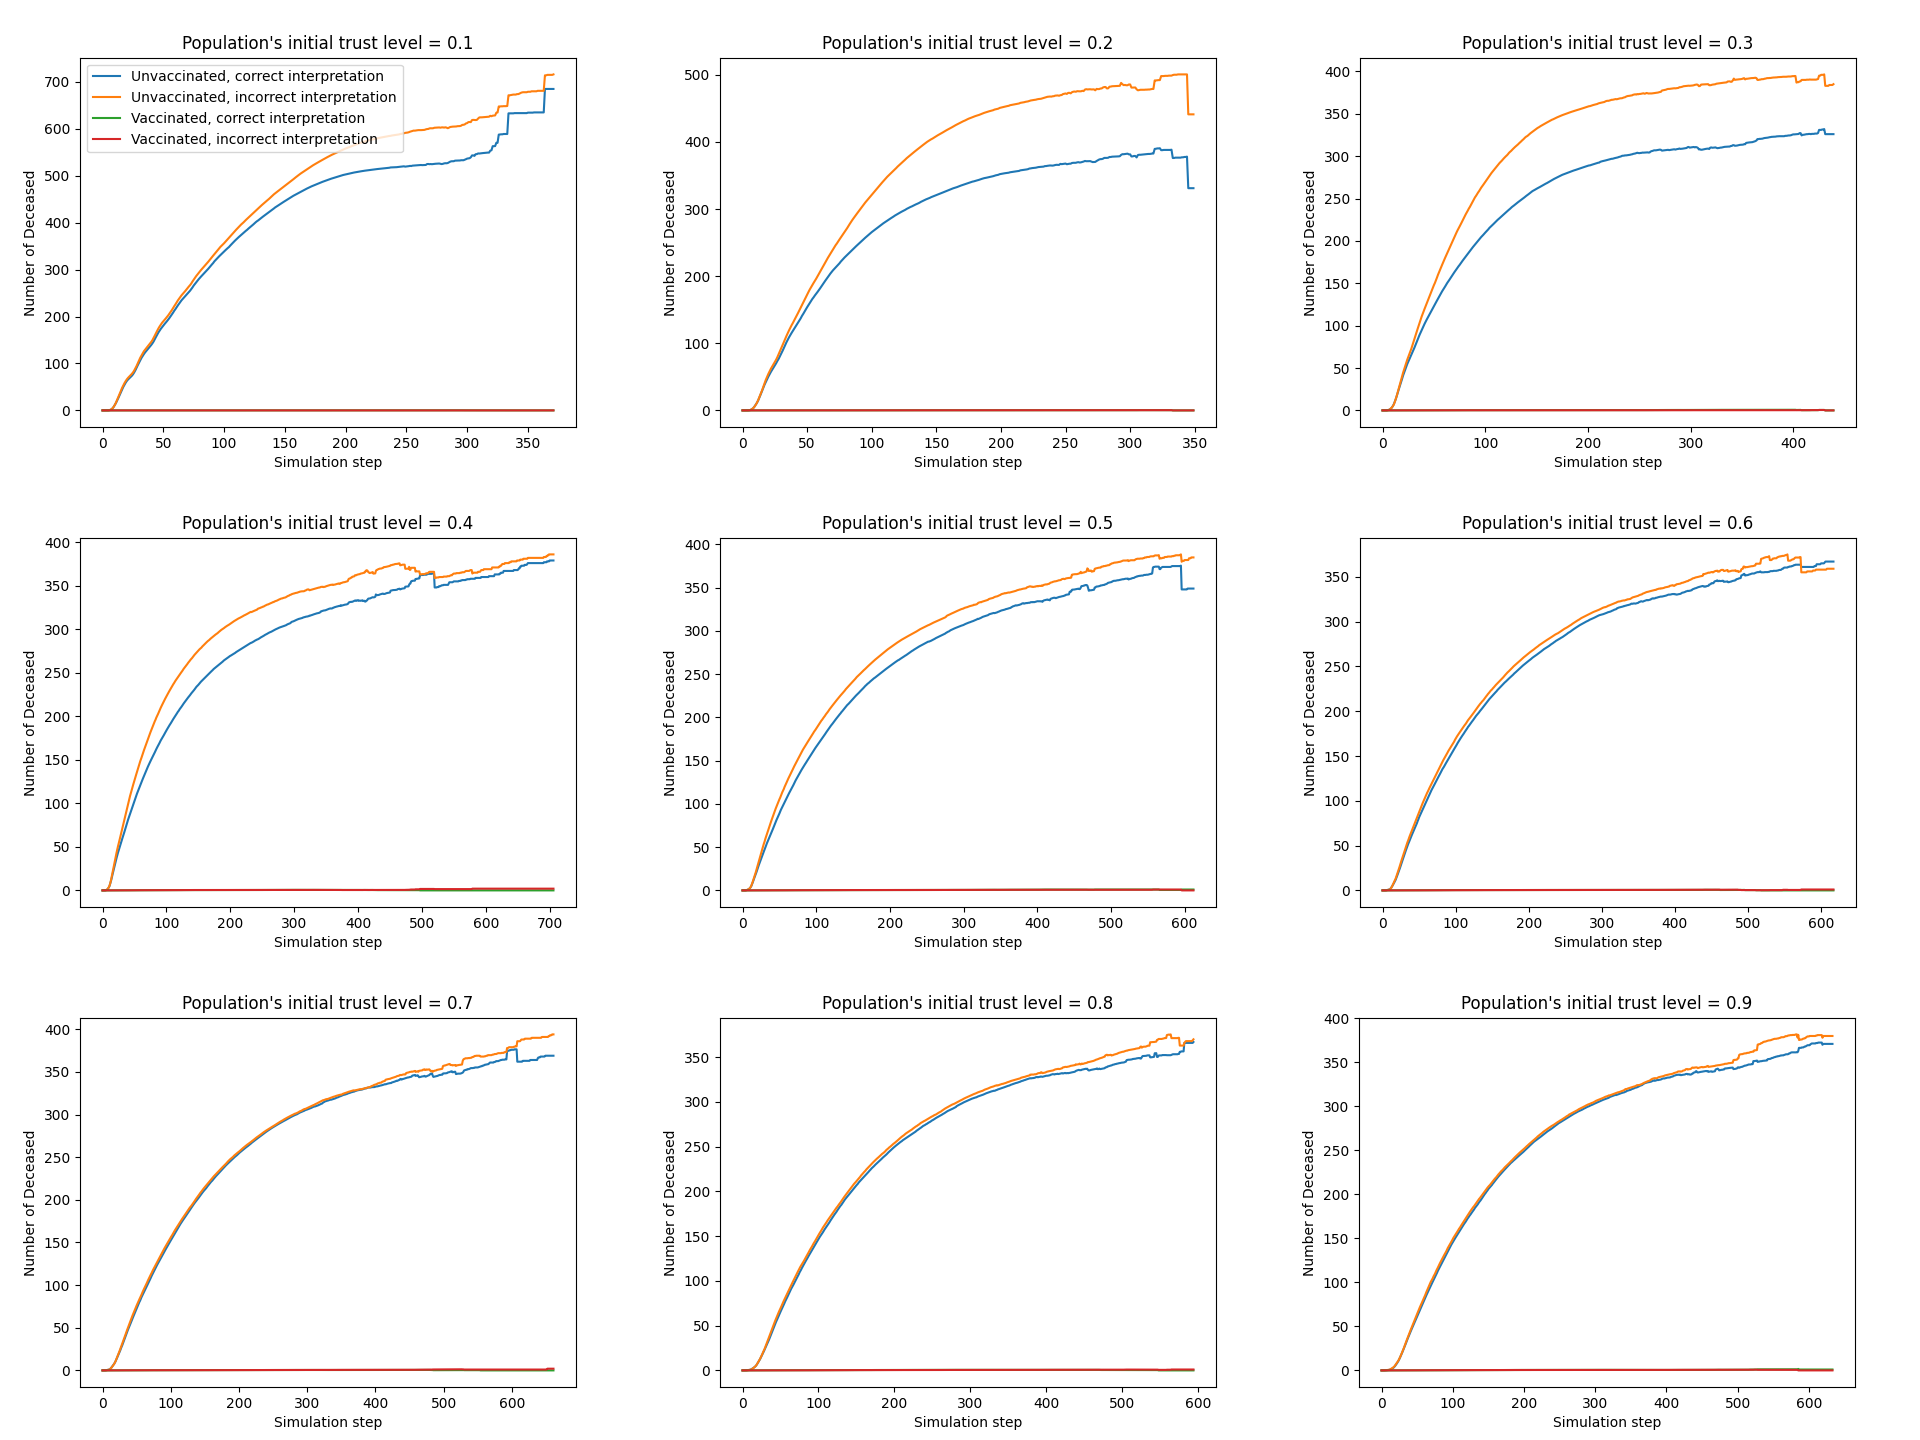
\includegraphics[width=1.3\linewidth, angle=90, origin=c]{pics/DVM.png}
    \endminipage
    \caption{Average number of deaths per vaccination and misinterpretation statuses at each simulation step for each population's initial trust level. The number of simulation steps (x-axis) is different between graphs.}
    \label{fig:dvm_landscape}
\end{figure}

\newpage

\begin{figure}[!htb]
    \centering
    \minipage{\textwidth}
        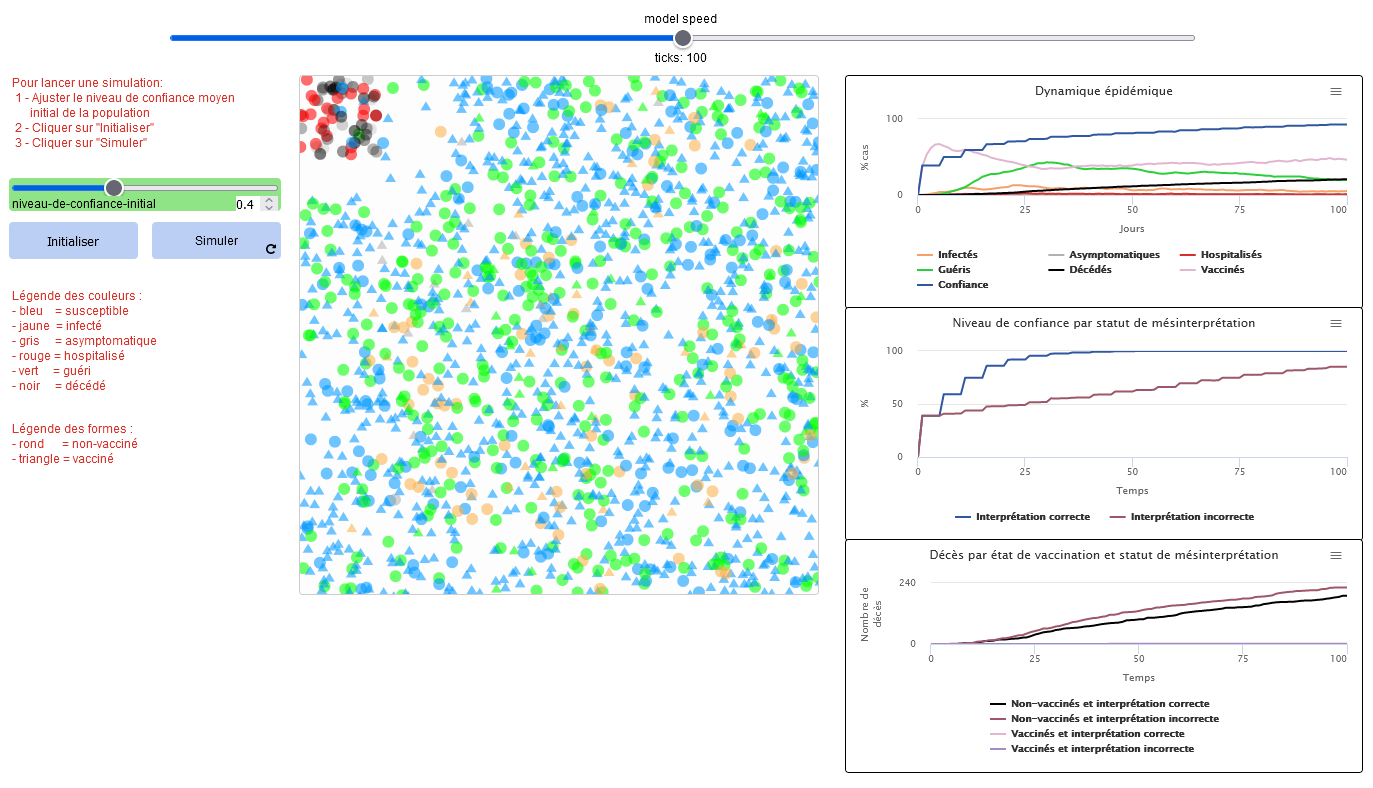
\includegraphics[width=1.4\linewidth, angle=90, origin=c]{pics/simulation_screenshot.png}
    \endminipage
    \caption{Screenshot of the simulation on NetLogo Web}
    \label{fig:simulation_screenshot}
\end{figure}

\newpage

%=========================================================


%=========================================================
\backmatter

%\bibliographystyle{plain} % plain-fr si rapport en français
%\bibliography{bibfile.bib}
\printbibliography[title={Articles}, type=article]
\printbibliography[title={Other sources}, nottype=article]

%\cleardoublepage % Goes to an odd page
%\pagestyle{empty} % no page number
%~\newpage % goes to a new even page

\end{document}